\documentclass{article}
\usepackage{graphicx} % Required for inserting images
\graphicspath{ {./images/} }
\graphicspath{ {images/} }
\usepackage{xcolor}
\usepackage{amsmath}
\usepackage{multicol}
\usepackage{amsmath}
\usepackage{amsfonts}
\usepackage{amssymb}
\usepackage{url}
\usepackage{mdframed}
\usepackage{hyperref}
\usepackage{subfigure}
\usepackage{vntex}
\usepackage{fancybox,graphicx}
\usepackage{mathrsfs} 
\usepackage{amsfonts}
\usepackage{longtable,array}
\usepackage{multirow}
\usepackage[latin1]{inputenc}
\usepackage{hyperref}
\newmdenv[linecolor=black,skipabove=\topsep,skipbelow=\topsep,
leftmargin=-5pt,rightmargin=-5pt,
innerleftmargin=5pt,innerrightmargin=5pt]{mybox}
\usepackage[a4paper,left=22mm,top=20mm,right=22mm]{geometry}
\title{Calculus II - Chapter 2\\Extremums of Functions of Several Variables}
\author{By HanLe from USTH LEARNING SUPPORT}
\date{April 2024}

\begin{document}

\maketitle
\tableofcontents
\newpage
\section{Directional Derivatives}
\subsection{Definition}
Directional derivatives help us find the \textbf{rate of change} of a function in the direction corresponding to unit vector $u = (u_1, u_2)$\\
This is the definition of directional derivative for \textbf{2-variable function}:\\
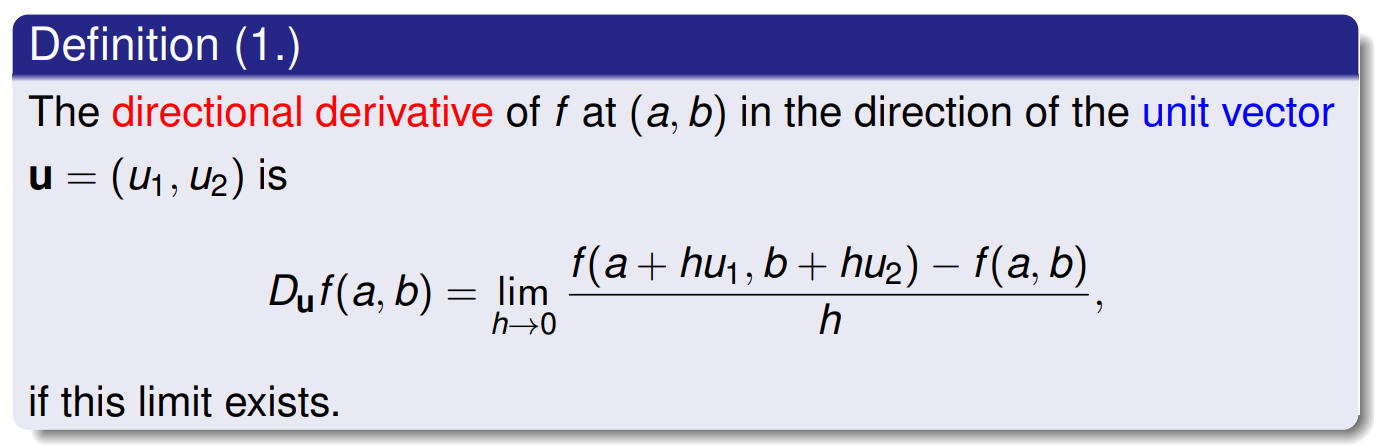
\includegraphics[width=1\linewidth]{image.png}
\textbf{Important:} If u is not a unit vector (a vector whose length is 1), then you have to normalize u before calculating the directional derivative.
\begin{center}
    Normalize u: $v=\displaystyle\frac{u}{||u||}$ (||u|| is the length of u)
\end{center}
The definition of directional derivative for \textbf{3-variable function}:\\
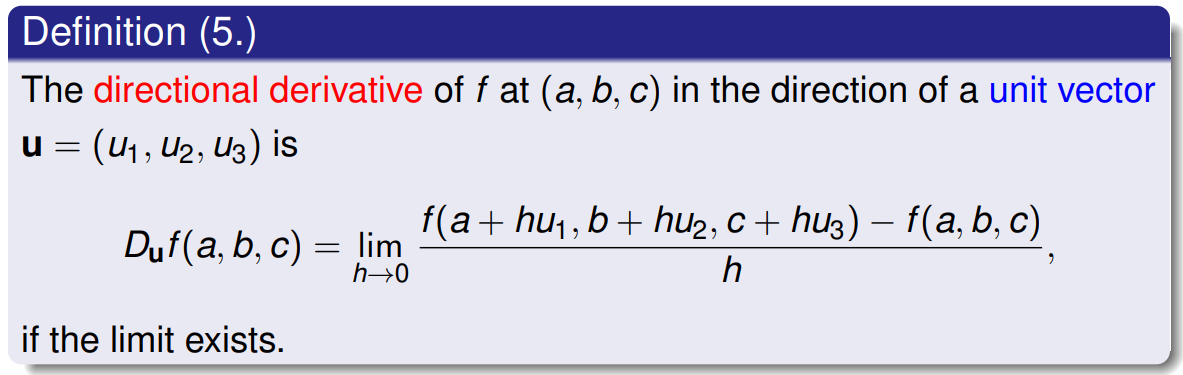
\includegraphics[width=1\linewidth]{1.1.png}
\textbf{Notice:} For a function of more than 3 variables, you can figure out the formula of definition by yourself.\\\\
\textbf{Example: } Find the derivative of $f(x,y)=xe^y+cos(xy)$ at $P_0=(2,0)$ in the direction $u=3i+4j$.
\begin{center}
    \textbf{Solution}
\end{center}
\textit{Recall: } $u=3i+4j$ means $u=(3,4)$\\
Normalize u: $v=\displaystyle\frac{u}{||u||}=\frac{(3,4)}{\sqrt{3^2+4^2}}=\frac{(3,4)}{5}=\left(\frac{3}{5},\frac{4}{5}\right)$
\begin{flalign*}
    D_uf(2,0)=D_vf(2,0)&=\displaystyle\lim_{h\rightarrow0}\frac{f(2+3h,0+4h)-f(2,0)}{h}\\
    &=\lim_{h\rightarrow0}\frac{\left(2+\displaystyle\frac{3}{5}h\right)e^{4h/5}+\cos\left[\left(2+\displaystyle\frac{3}{5}h\right).\displaystyle\frac{4}{5}h\right]-(2e^0+\cos 0)}{h}\\
    &=\displaystyle\lim_{h\rightarrow0}\frac{\left(2+\displaystyle\frac{3}{5}h\right)e^{4h/5}+\cos\left[\left(2+\displaystyle\frac{3}{5}h\right).\displaystyle\frac{4}{5}h\right]-3}{h}
\end{flalign*}
If we try to substitute $h=0$ to calculate this limit, it will be the form $\displaystyle\frac{0}{0}$, so we will apply L'Hospital's Rule.
\begin{flalign*}
    D_uf(2,0)&=\displaystyle\lim_{h\rightarrow0}\left(\frac{3}{5}e^{4h/5}+\frac{4}{5}e^{4h/5}\left(2+\frac{3}{5}h\right)-\sin \left[\left(2+\frac{3}{5}h\right).\frac{4}{5}h\right]\left[\frac{3}{5}.\frac{4}{5}h+\frac{4}{5}\left(2+\frac{3}{5}h\right)\right]\right)\\
    &=\displaystyle\frac{3}{5}+\frac{4}{5}.2-\sin(0).\frac{4}{5}.2\\
    &=\displaystyle\frac{11}{5}
\end{flalign*}
You can see that calculating the derivative by definition takes us so much time. However, we have another way to calculate it, let's see that way in section 1.2.
\subsection{Find Directional Derivatives by Dot Product and Gradient Vector}
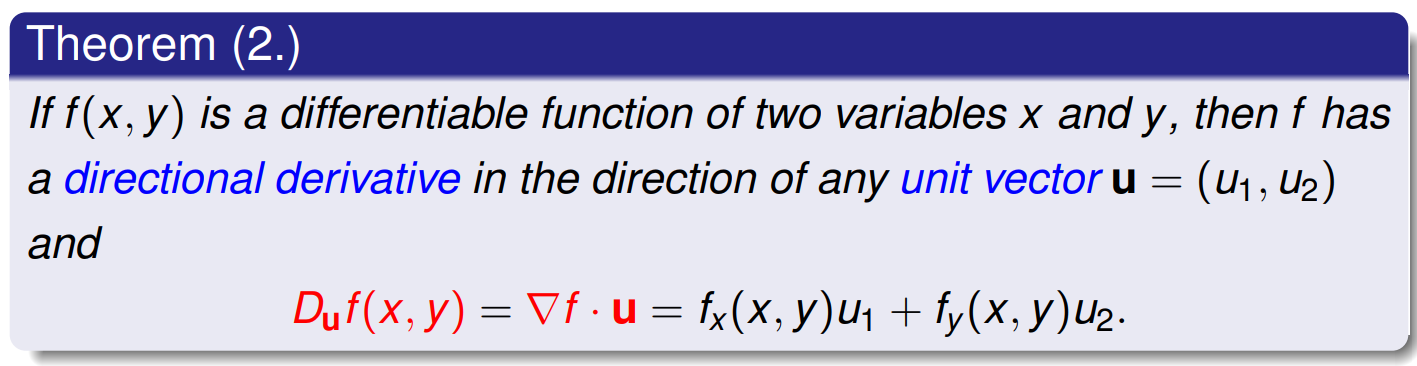
\includegraphics[width=1\linewidth]{1.2.png}
\textbf{Important: }Like the definition, if u is not a unit vector (a vector whose length is 1), then you have to normalize u before calculating the directional derivative.\\\\
Let's calculate the derivative in section 1.1 this way to see how fast it is:\\
\textbf{Example: } Find the derivative of $f(x,y)=xe^y+cos(xy)$ at $P_0=(2,0)$ in the direction $u=3i+4j$.
\begin{center}
    \textbf{Solution}
\end{center}
In section 1.1, u is normalized and becomes $v=\displaystyle\left(\frac{3}{5},\frac{4}{5}\right)$\\
We have:
\begin{flalign*}
    f_{x}(x,y)=&e^y-y\sin(xy)&\\
    f_{y}(x,y)=&xe^y-x\sin(xy)&
\end{flalign*}
$   \Rightarrow \nabla f(x,y)=(f_x,f_y)=(e^y-y\sin(xy),xe^y-x\sin(xy))\\
    \Rightarrow \nabla f(2,0)=(1,2)\\\\
    \Rightarrow D_uf(2,0)=D_vf(2,0)=\nabla f(2,0).v=(1,2).\displaystyle\left(\frac{3}{5},\frac{4}{5}\right)=1.\frac{3}{5}+2.\frac{4}{5}=\frac{3}{5}+\frac{8}{5}=\frac{11}{5}
    $\\
\textbf{Example: }Let u be the unit vector in $R^2$ given by angle $\theta=\displaystyle\frac{\pi}{3}$. Find the directional derivative of $f(x,y)=x^3-3xy+4y^2$ in the direction u.
\begin{center}
    \textbf{Solution}
\end{center}
The unit vector u given by angle $\theta=\displaystyle\frac{\pi}{3}$ means $u=\cos \displaystyle\left(\frac{\pi}{3}\right)\hat{i}+\sin\left(\frac{\pi}{3}\right)\hat{j}=\frac{1}{2}i+\frac{\sqrt{3}}{2}j$\\
\textbf{Note:}\\
- Chiếu vector u xuống Ox thì ra $\cos\displaystyle\left(\frac{\pi}{3}\right)\hat{i}$ và chiếu vector u xuống Oy thì ra $\sin\displaystyle\left(\frac{\pi}{3}\right)\hat{j}$ \\
- $\hat{i}$ và $\hat{j}$ là các unit vector ứng với Ox,Oy\\
- u ở trường hợp này luôn là unit vector vì với mọi $\theta$ ta có $||u||=\sqrt{sin^2\theta+cos^2\theta}=1$\\
$\Rightarrow u=\displaystyle\left(\frac{1}{2},\frac{\sqrt{3}}{2}\right)$\\
You can see the unit vector u in the figure below to understand what it looks like.
\begin{center}
    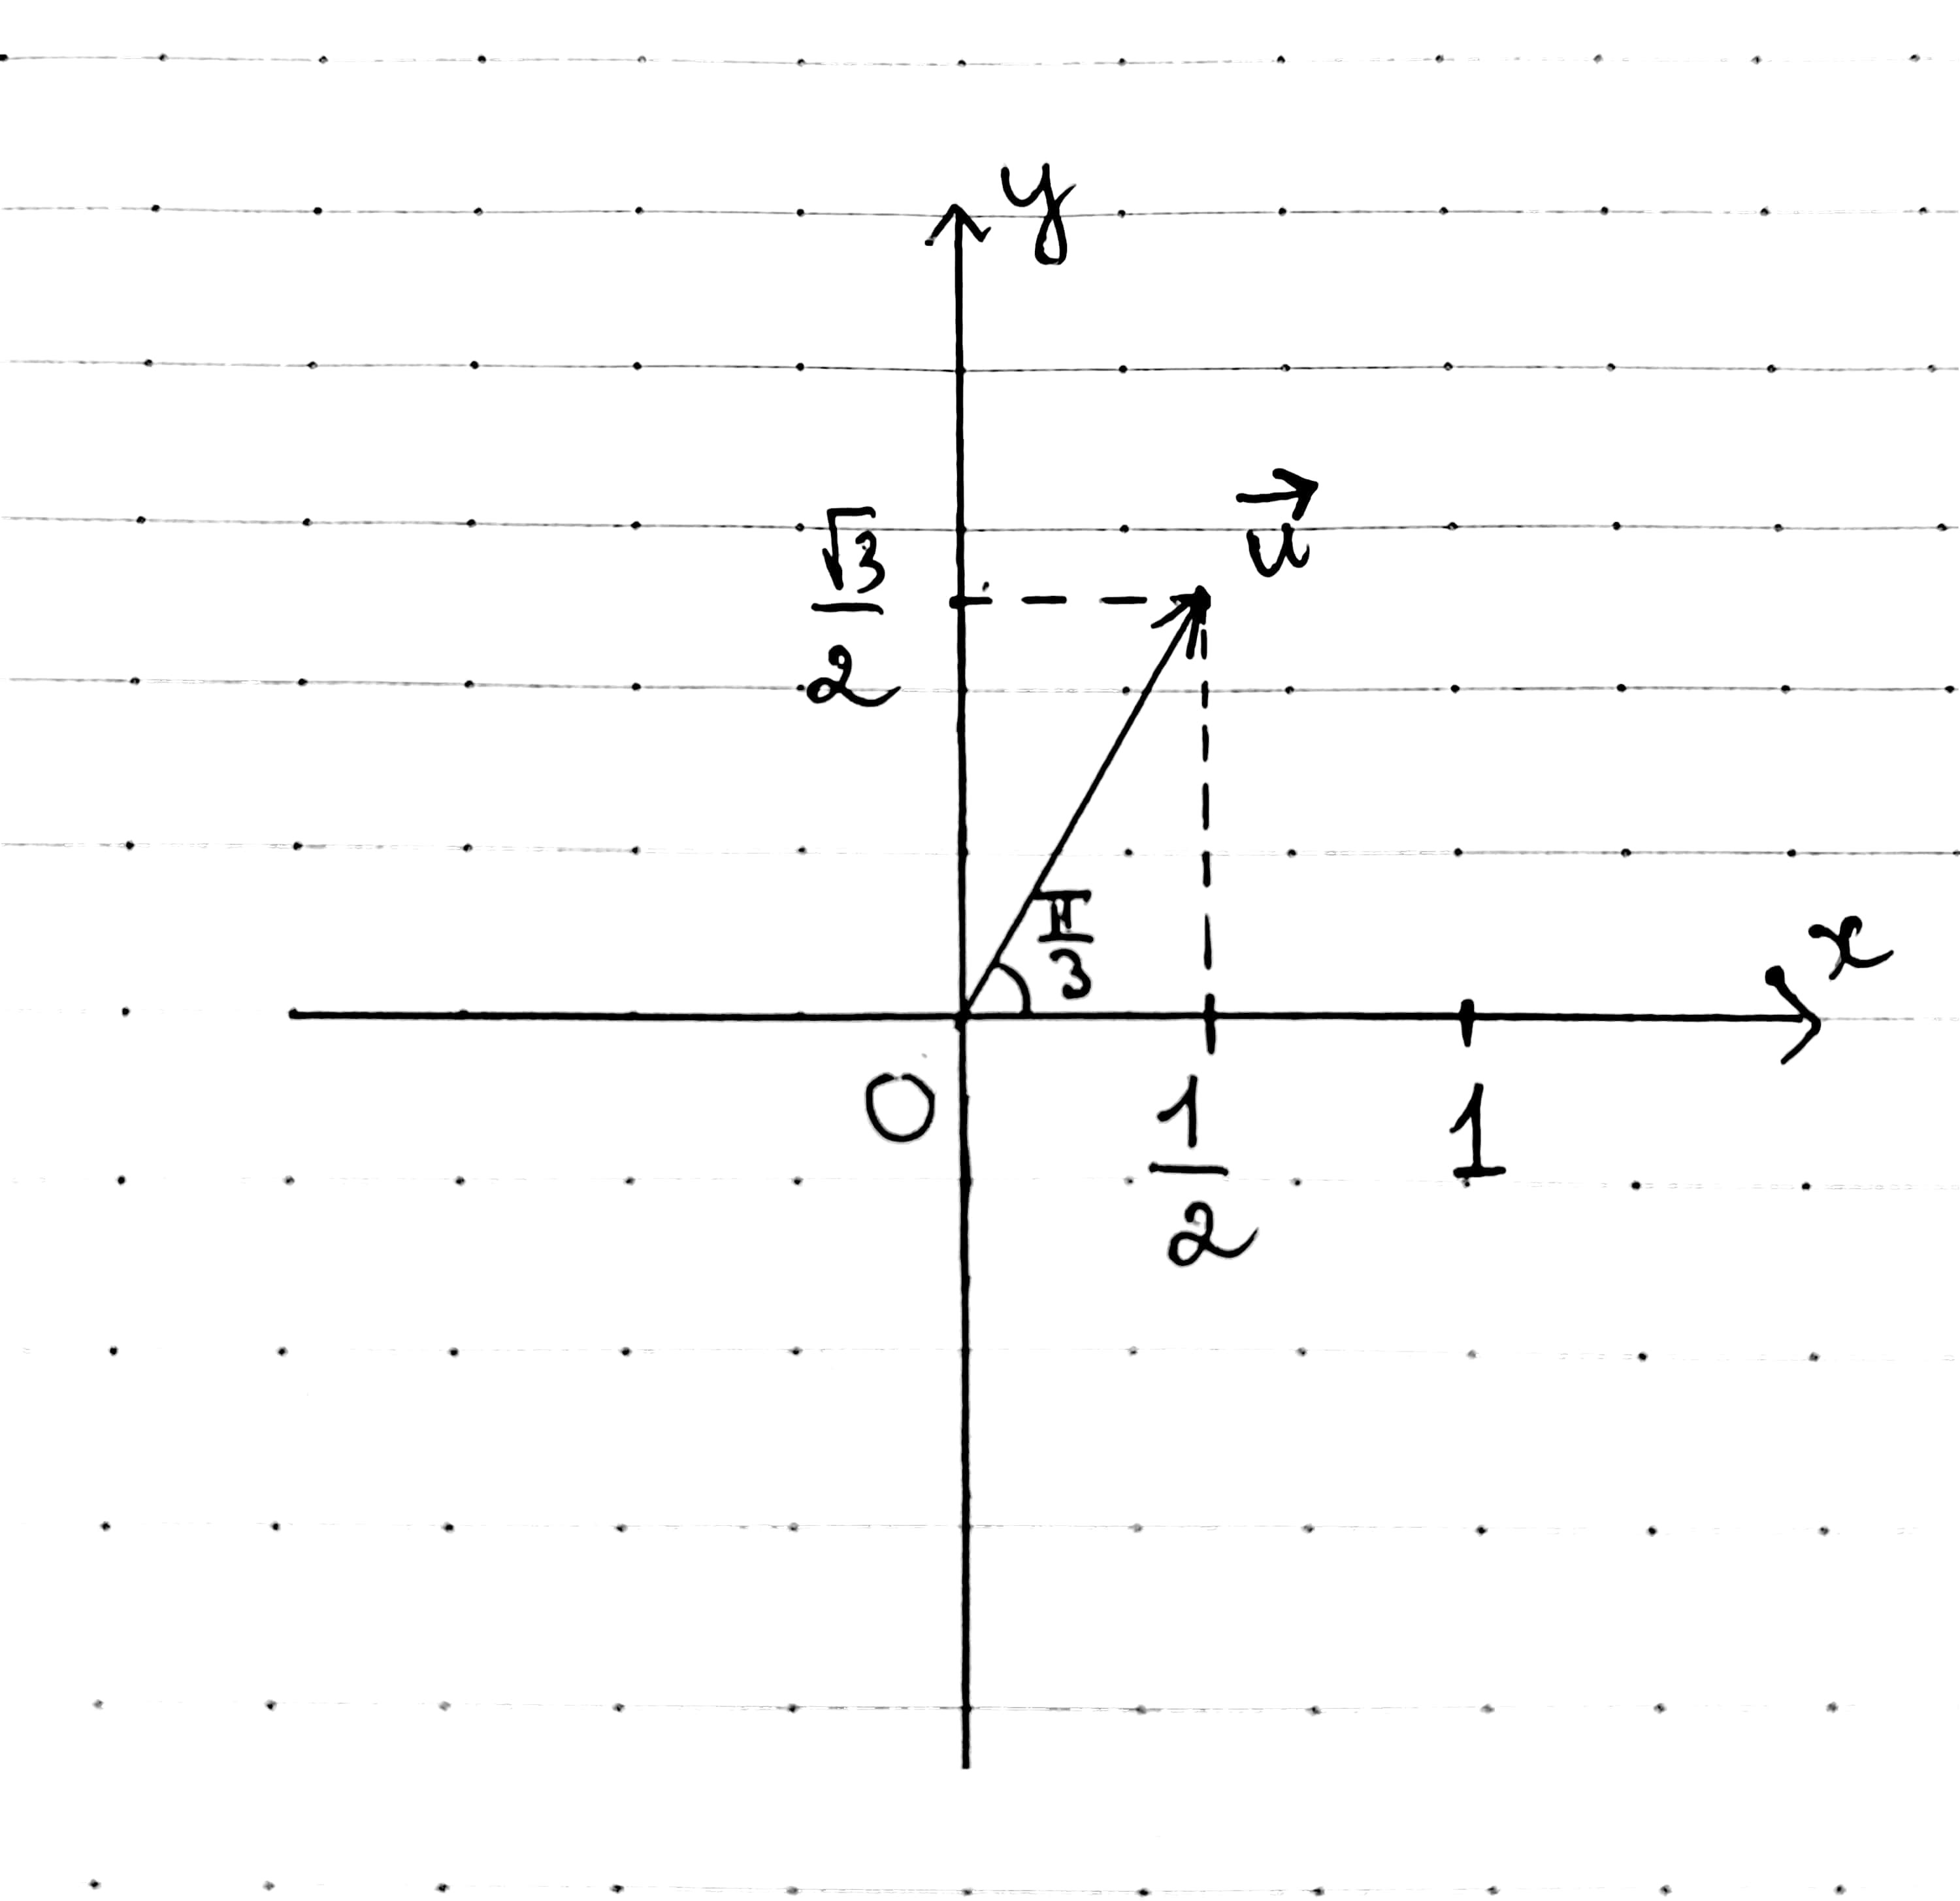
\includegraphics[width=0.5\linewidth]{vectoru.png}
\end{center}
We have:
\begin{flalign*}
    f_x&=3x^2-3y\\
    f_y&=-3x+8y
\end{flalign*}
    $\Rightarrow\nabla f(x,y)=(3x^2-3y,-3x+8y)\\
    \Rightarrow D_uf(x,y)=(3x^2-3y,-3x+8y).\displaystyle\left(\frac{1}{2},\frac{\sqrt{3}}{2}\right)=\frac{3}{2}x^2-\frac{3}{2}y-\frac{3\sqrt{3}}{2}x+4\sqrt{3}y$
\section{Maximum and Minimum Rate of Change}
\textbf{Recall:} The directional derivative describes the rate of change of a function in the direction corresponds to the unit vector u.\\
These are the cases when the rate of change in f is maximum or minimum:\\
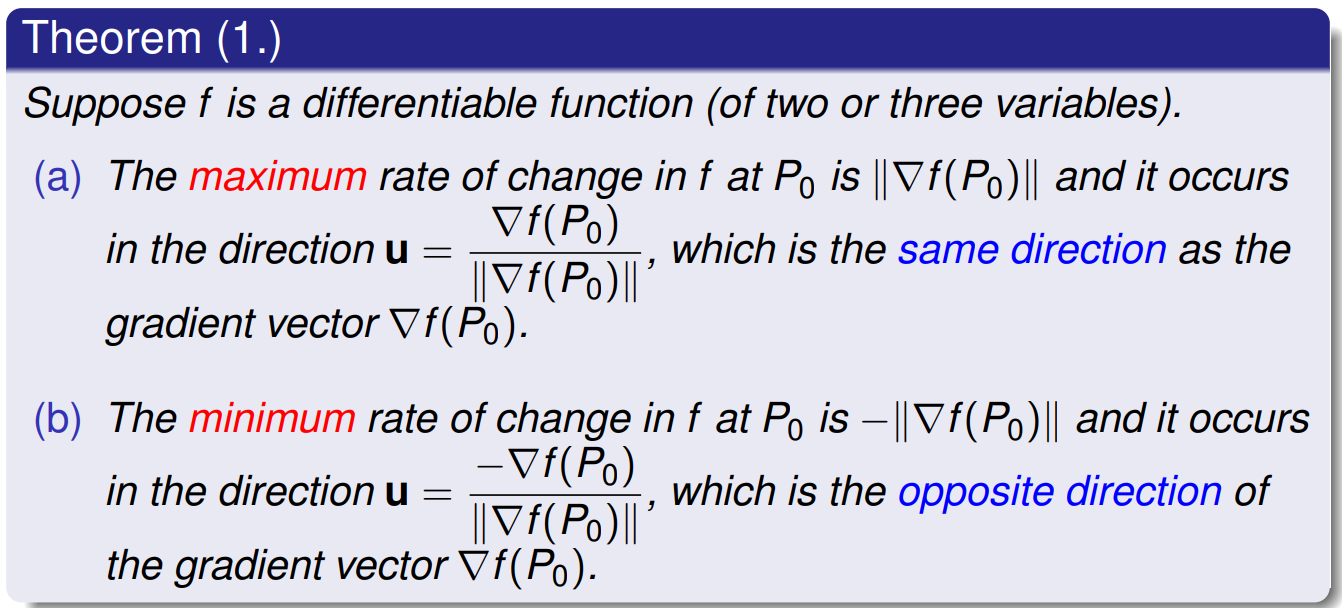
\includegraphics[width=1\linewidth]{2.png}
\textbf{Important: }\\
- The gradient vector $\nabla f$ is orthogonal to the level curve $f(x, y) = k$ and it is the direction where f increases most rapidly (largest rate)\\
- The gradient vector $\nabla F$ is orthogonal to the level surface
$F(x, y, z) = k$ and it is the direction where F increases most
rapidly (largest rate).\\
\textbf{Example: }Find the directions in which $f(x,y)=xe^y$:\\
a) increases most rapidly at (2,0) and the rate of change corresponds to this direction. (maximum)\\
b) decreases most rapidly at (2,0) and the rate of change corresponds to this direction. (minimum)
\begin{center}
    \textbf{Solution}
\end{center}
We have:\\
$f_x=e^y$ and 
$f_y=xe^y$ 
$\Rightarrow\nabla f(x,y)=(e^y,xe^y)$ \\
$\Rightarrow\nabla f(2,0)=(1,2)$\\
$\Rightarrow||\nabla f(2,0)||=\sqrt{1^2+2^2}=\sqrt{5}$\\
a) The rate of change at (2,0) corresponds to this direction is:
\begin{center}
    $D_uf(2,0)=||\nabla f(2,0)||=\sqrt{5}$
\end{center}
The direction is:
\begin{center}
    $u=\displaystyle\frac{\nabla f(2,0)}{||\nabla f(2,0)||}=\frac{(1,2)}{\sqrt{5}}=\left(\frac{1}{\sqrt{5}},\frac{2}{\sqrt{5}}\right)$
\end{center}
\textit{Thử lại:} $D_uf(2,0)=\nabla f(2,0).u=(1,2).\displaystyle\left(\frac{1}{\sqrt{5}},\frac{2}{\sqrt{5}}\right)=\frac{1}{\sqrt{5}}+\frac{4}{\sqrt{5}}=\frac{5}{\sqrt{5}}=\sqrt{5}$\\
b) The rate of change at (2,0) corresponds to this direction is:
\begin{center}
    $D_uf(2,0)=-||\nabla f(2,0)||=-\sqrt{5}$
\end{center}
The direction is:
\begin{center}
    $u=\displaystyle-\frac{\nabla f(2,0)}{||\nabla f(2,0)||}=-\frac{(1,2)}{\sqrt{5}}=-\left(\frac{1}{\sqrt{5}},\frac{2}{\sqrt{5}}\right)=\left(-\frac{1}{\sqrt{5}},-\frac{2}{\sqrt{5}}\right)$
\end{center}
\section{Local Extreme Values}
\subsection{Definition}    
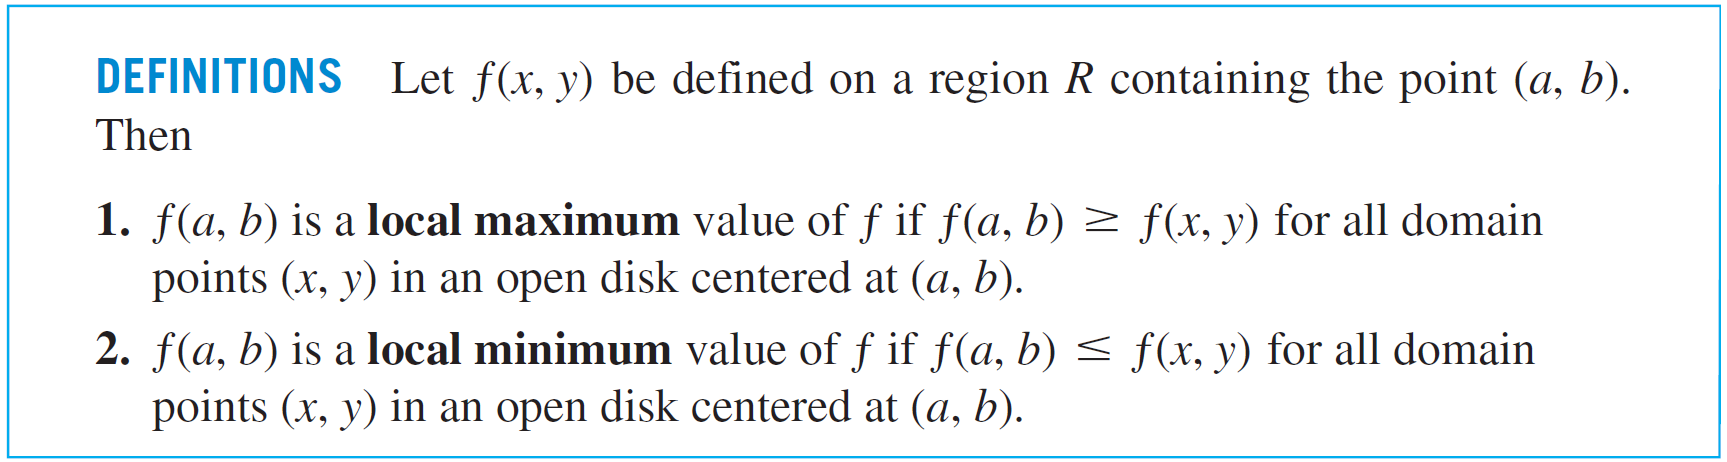
\includegraphics[width=1\linewidth]{2.2.png}\\
You can observe these figures to imagine better:\\
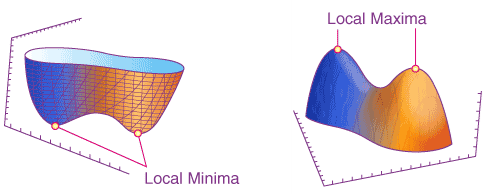
\includegraphics[width=0.6\linewidth]{3.222.png}
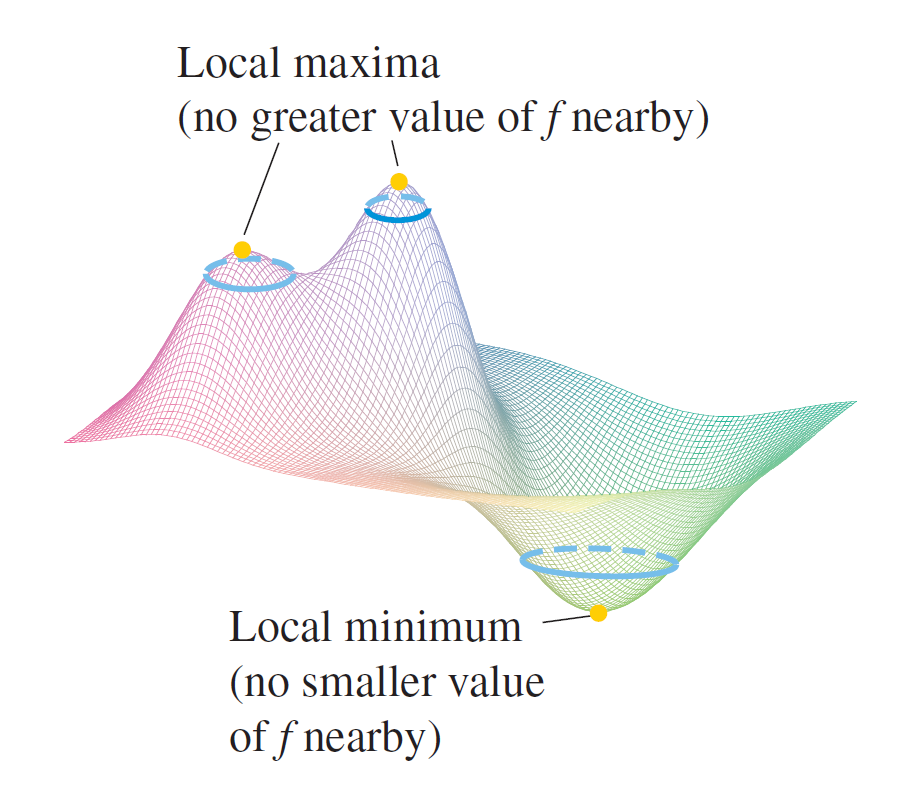
\includegraphics[width=0.4\linewidth]{3.22.png}\\
\subsection{Critical point and saddle point}
\subsubsection{Critical point: singular point and stationary point}
These are the definitions of critical point, singular point, and stationary point of a 2-variable function:\\
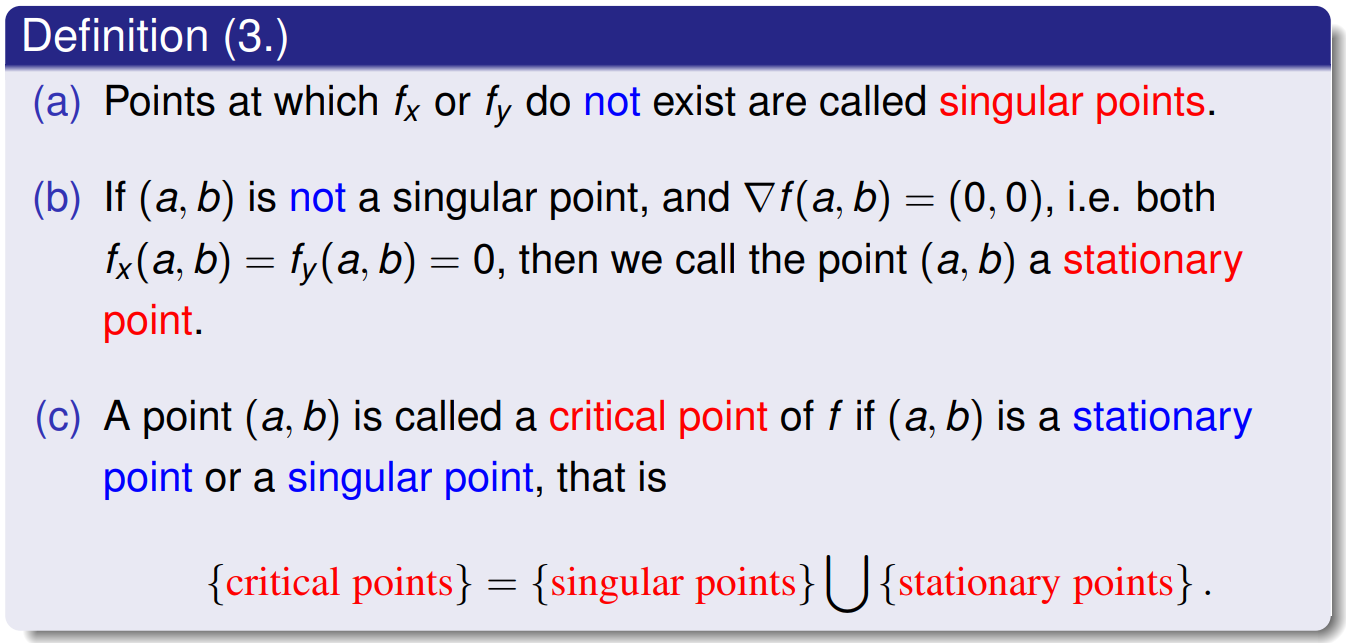
\includegraphics[width=1\linewidth]{3.1.png}
\textbf{Note: }\\
- The definitions of critical point, singular point, and stationary point of other multi-variable functions are similar to those of 2-variable function.\\
- The critical point of a multi-variable function is similar to that of a 1-variable function.\\
\textbf{Example: }Find all critical points of $f(x,y)=\displaystyle e^{x\sqrt[3]{y}-x^2}$
\begin{center}
    \textbf{Solution}
\end{center}
We have:\\
$
f_x=e^{x\sqrt[3]{y}-x^2}(\sqrt[3]{y}-2x)\\
f_y=e^{x\sqrt[3]{y}-x^2}.\displaystyle\frac{x}{3\sqrt[3]{y^2}}
$ (Biến $\sqrt[3]{y}=y^{1/3}$ để đạo hàm)\\
$\Rightarrow f_y$ is not defined when $y=0$ \\
$\Rightarrow$ For all $x\in R$, $(x,0)$ are singular points of f\\
With $y\ne 0$, consider $
\left\{
\begin{array}{c}
     f_x=0  \\
     f_y=0
\end{array}
\right.\\
\iff\left\{
\begin{array}{cr}
     e^{x\sqrt[3]{y}-x^2}(\sqrt[3]{y}-2x)&=0  \\
     e^{x\sqrt[3]{y}-x^2}.\displaystyle\frac{x}{3\sqrt[3]{y^2}}&=0
\end{array}
\right.\\
\iff\left\{
\begin{array}{cr}
     \sqrt[3]{y}-2x&=0  \\
     \displaystyle\frac{x}{3\sqrt[3]{y^2}}&=0
\end{array}
\right.\\
\iff \left\{
\begin{array}{cr}
     x=0  \\
     y=0
\end{array}
\right.
$
(not suitable)\\
$\Rightarrow f$ does not have any stationary points\\
$\Rightarrow (x,0)$ $(x \in R)$ are critical points of $f$ 
\subsubsection{Saddle point}
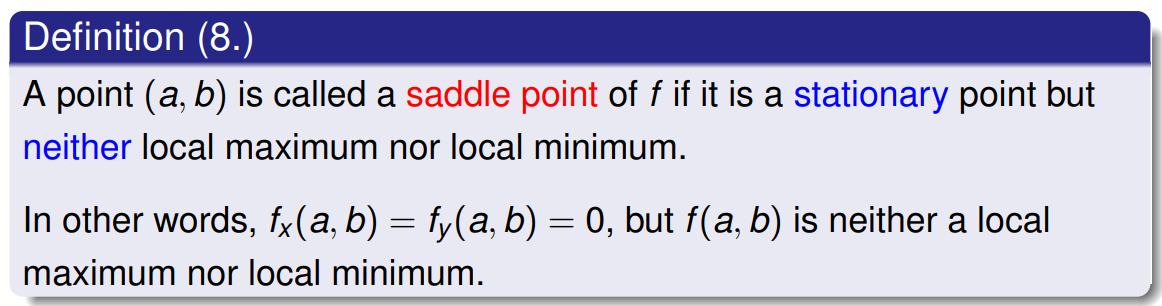
\includegraphics[width=1\linewidth]{3.2.2.png}\\ 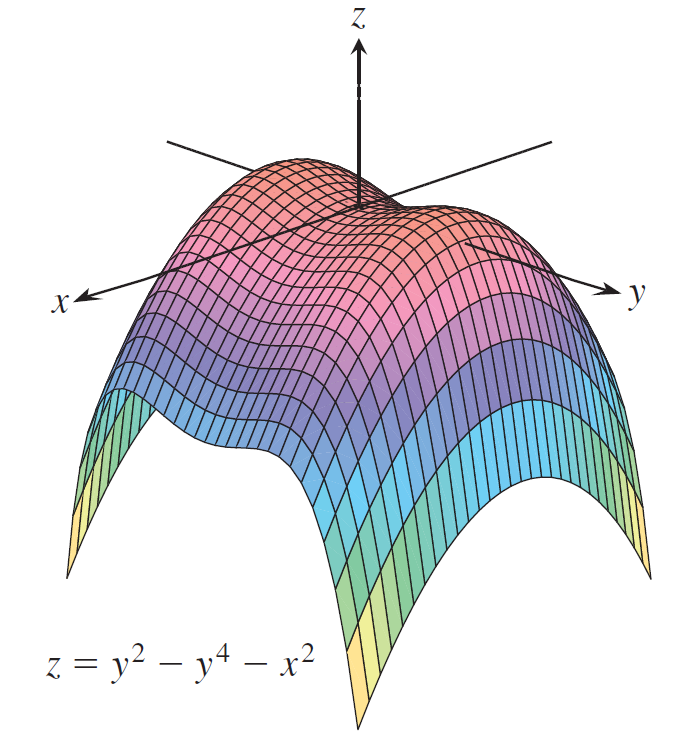
\includegraphics[width=0.5\linewidth]{3.2.22.png}    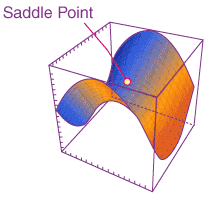
\includegraphics[width=0.5\linewidth]{3.2.23.png}
\subsection{Derivative Test for Local Extreme Values}
\subsubsection{First Derivative Test for Local Extreme Values}
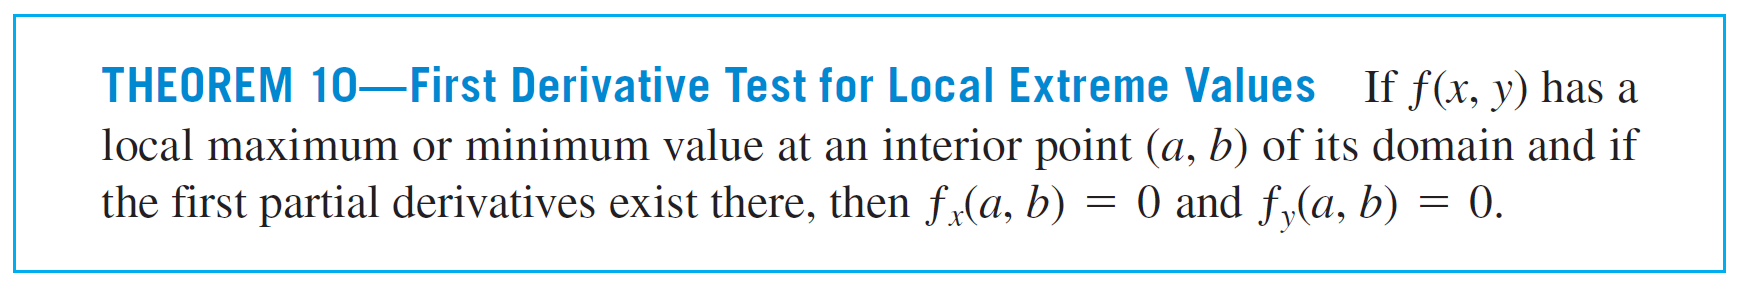
\includegraphics[width=1\linewidth]{3.3.png}\\
\textbf{Notice: } This is just the necessary condition (not sufficient condition) for a function to have a local extreme value at the point (a,b). \\
$\Rightarrow$\textit{ Explanation:} If $f_x(a,b)=0$ and $f_y(a,b)=0$ then (a,b) will be a stationary point. However, a stationary point can be a local extremum or a saddle point. Therefore, you can not conclude what $f(a,b)$ is, you have to consider the Second Derivative Test below.\\
\textbf{Notice (Vietnamese version for better understand):} Đây chỉ là điều kiện cần (chưa phải điều kiện đủ) để hàm số có cực trị tại điểm (a,b).\\
$\Rightarrow$ \textit{Giải thích:} Nếu $f_x(a,b)=0$ và $f_y(a,b)=0$ thì (a,b) sẽ là một stationary point. Tuy nhiên một stationary point có thể là một điểm cực trị hoặc là một saddle point. Cho nên, bạn không thể kết luận luôn $f(a,b)$ là gì mà phải xét đến Second Derivative Test dưới đây.
\subsubsection{Second Derivative Test for Local Extreme Values}
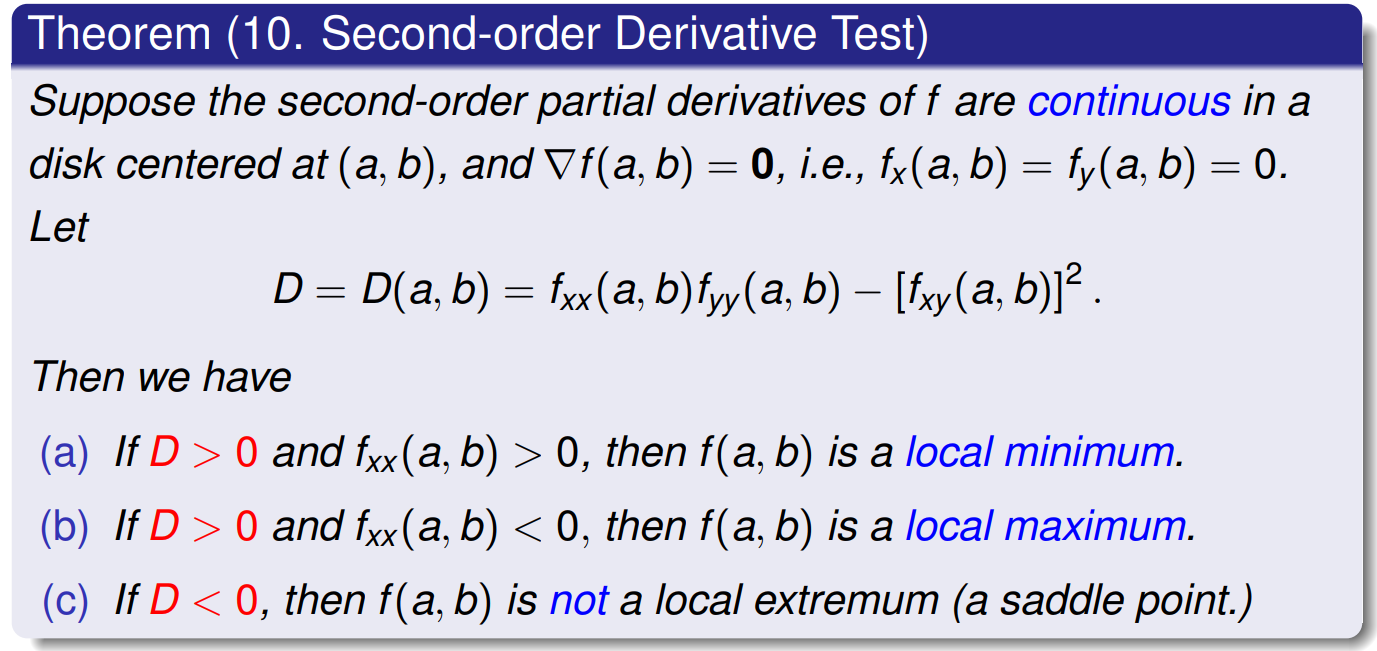
\includegraphics[width=1\linewidth]{3.4.png}
\textbf{Notice: }\\
- If $D=0$, the test is inconclusive. Therefore, you have to some other way to determine the behavior of $f$ at $(a,b)$.\\
- Another way to remember $D(a,b)=f_{xx}(a,b)f_{yy}(a,b)-[f_{xy}(a,b)]^2$ is writing it in determinant form:
\begin{equation*}
    D(a,b)=
    \begin{vmatrix}
        f_{xx}&f_{xy}\\
        f_{xy}&f_{yy}
    \end{vmatrix}
\end{equation*}
\textbf{Example:} Find all the local maximum and minimum values of $f(x,y)=y^2-y^4-x^2$
\begin{center}
    \textbf{Solution}
\end{center}
First, we have to find all stationary points of $f$ by the First Derivative Test.\\
We have:\\
$f_x=-2x\\
f_y=2y-4y^3$\\
Consider $\left\{
\begin{array}{c}
     f_x=0  \\
     f_y=0
\end{array}
\right.
\iff\
\left\{
\begin{array}{cr}
     -2x&=0  \\
     2y-4y^3&=0
\end{array}
\right.
\iff\
\left\{
\begin{array}{cr}
     x=0  \\
     \left[
     \begin{array}{cr}
        y=\pm \displaystyle\frac{\sqrt{2}}{2}\\
        y=0
     \end{array}
     \right.
\end{array}
\right.
\iff
\left[
\begin{array}{cr}
     \left\{
     \begin{array}{cr}
        x=0\\
        y=\pm \displaystyle\frac{\sqrt{2}}{2}
     \end{array}
     \right.\\
     \left\{
     \begin{array}{cr}
        x=0\\
        y=0
     \end{array}
     \right.
\end{array}
\right.\\
\Rightarrow \left(0,\displaystyle\frac{\sqrt{2}}{2}\right),\left(0,\displaystyle\frac{-\sqrt{2}}{2}\right),(0,0)$ are stationary points of $f(x,y)$\\
Now using the Second Derivative Test to consider if those stationary points are local extremums.\\
We have:\\
$
f_{xx}=-2\\
f_{yy}=2-12y^2\\
f_{xy}=0\\
\Rightarrow D(x,y)=
    \begin{vmatrix}
        f_{xx}&f_{xy}\\
        f_{xy}&f_{yy}
    \end{vmatrix}
    =f_{xx}f_{yy}-{f_{xy}}^2=-2(2-12y^2)=24y^2-4
$\\
We have:\\
+) $D\left(0,0\right)=-4\\
\Rightarrow (0,0)$ is a saddle point.
\\
+) $
    D\left(0,\displaystyle\frac{\sqrt{2}}{2}\right)=24.\left(\displaystyle\frac{\sqrt{2}}{2}\right)^2-1=8>0 
$ and $f_{xx}<0 \\\Rightarrow f\left(0,\displaystyle\frac{\sqrt{2}}{2}\right)=\displaystyle\frac{1}{4}$ is a local maximum.\\
+) $
    D\left(0,\displaystyle\frac{-\sqrt{2}}{2}\right)=24.\left(\displaystyle\frac{-\sqrt{2}}{2}\right)^2-1=8>0 
$ and $f_{xx}<0 \\\Rightarrow f\left(0,\displaystyle\frac{-\sqrt{2}}{2}\right)=\displaystyle\frac{1}{4}$ is a local maximum.\\
\textbf{Example:} Find all the local maximum and minimum values of $f(x,y)=xy-x^2-y^2-2x-2y+4$.
\begin{center}
    \textbf{Solution}
\end{center}
We have:\\
$f_x=y-2x-2\\
f_y=x-2y-2$\\
Consider
$\left\{
\begin{array}{cr}
     f_x=0\\
     f_y=0
\end{array}
\right.
\iff
\left\{
\begin{array}{cr}
     y-2x-2=&0  \\
     x-2y-2=&0 
\end{array}
\right.
\iff
\left\{
\begin{array}{cr}
    y-2(2y+2)-2=0&  \\
    x=2y+2
\end{array}
\right.\\
\iff
\left\{
\begin{array}{cr}
    y-2(2y+2)-2=0  \\
    x=2y+2
\end{array}
\right.
\iff
\left\{
\begin{array}{cr}
    y=-2  \\
    x=-2
\end{array}
\right.\\
\Rightarrow (-2,-2)$ is the stationary point of $f$\\
We have:\\
  $f_{xx}=-2\\
    f_{yy}=-2\\
    f_{xy}=1$\\
$D(-2,-2)=f_{xx}f_{yy}-{f_{xy}}^2=4-1=3>0$ and $f_{xx}<0\\
\Rightarrow f(-2,-2)=8$ is the local maximum of $f$
\section{Absolute Extreme Values}
\subsection{Definition}
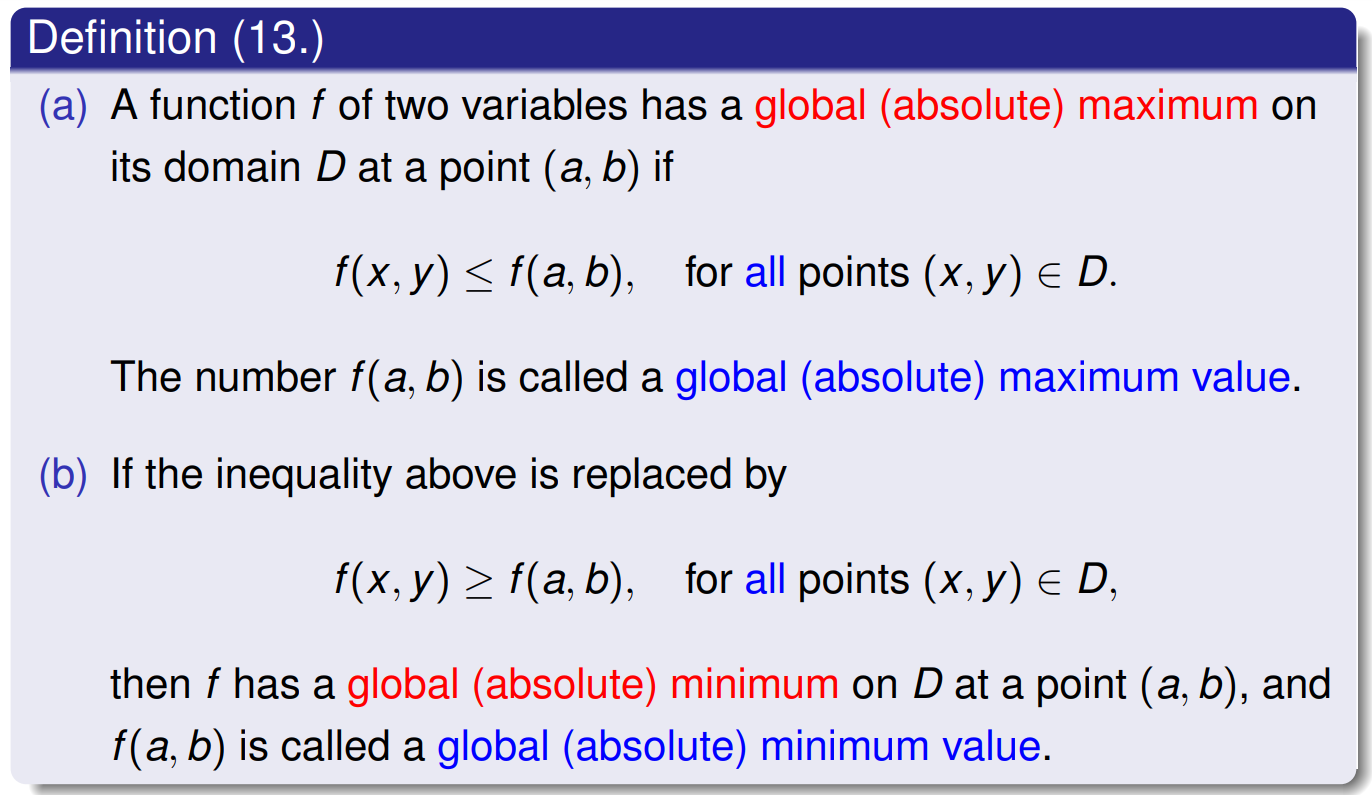
\includegraphics[width=1\linewidth]{4.png}\\
You can observe these figures to imagine better:
\\
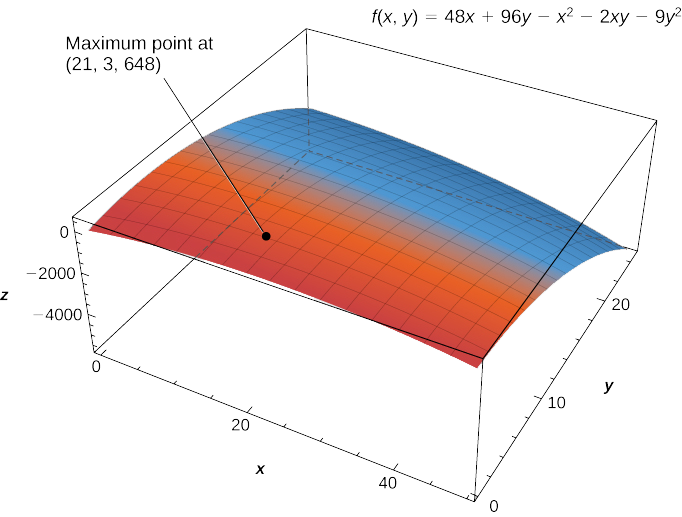
\includegraphics[width=0.5\linewidth]{4.1.png}    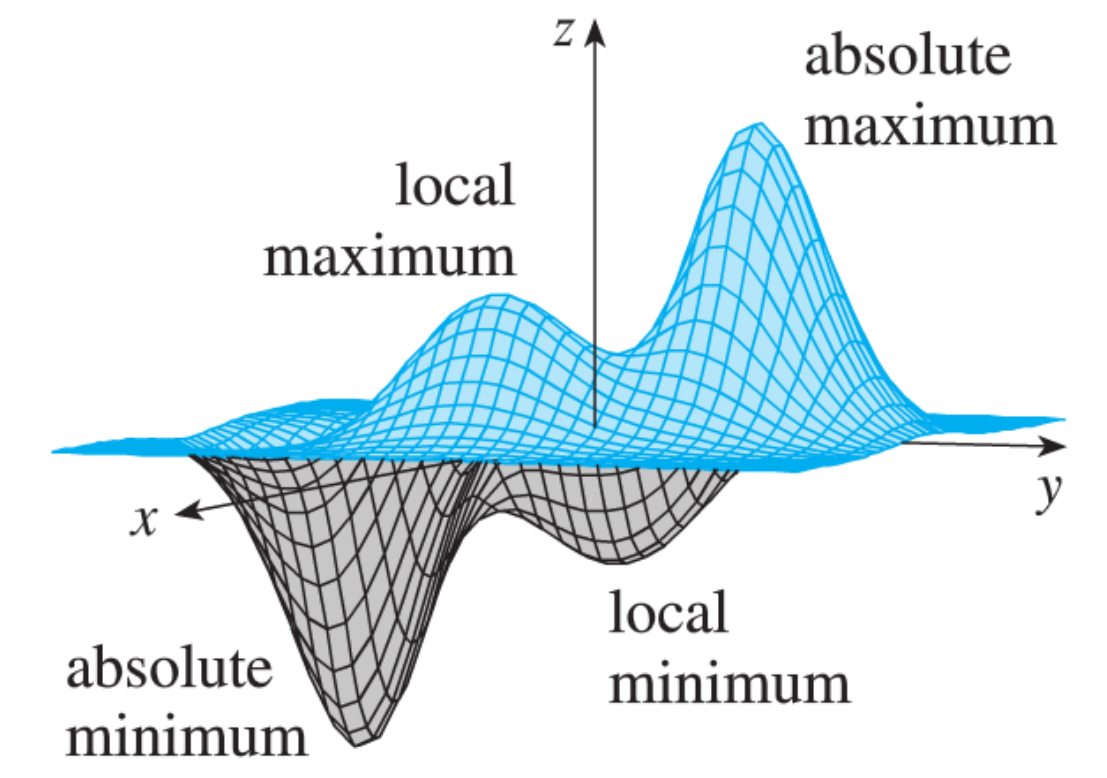
\includegraphics[width=0.5\linewidth]{4.12.png}
\subsection{Find Absolute Maximum and Minimum Values on closed bounded regions}   
\begin{mybox}
We can find the absolute extrema of a continuous function $f(x,y)$ in its closed, bounded domain D in 4 steps:
\begin{enumerate}
    \item Sketch the domain D.
    \item List all \textbf{critical point}s of $f$ in its domain and evaluate the values of $f$ at those points.
    \item List all \textbf{boundary points} where $f$ may have absolute maximum and minimum values and evaluate the values of $f$ at those points. (Gồm các local extreme và đầu mút)
    \item Look at all values of $f$ at points evaluated in two previous steps then choose the maximum and minimum values.
\end{enumerate}
\end{mybox}
\textit{(Ta có thể thấy là các bước khá giống với việc tìm Max và Min của hàm một biến)}\\
\textbf{Example:} Find the absolute maximum and minimum values of $f(x,y)=2x^2-4x+y^2-4y+1$ on the closed triangular (hình tam giác) plate bounded by the lines $x=0,y=2,y=2x$ in the first quadrant (góc phần tư thứ nhất).
\begin{center}
    \textbf{Solution}\\
    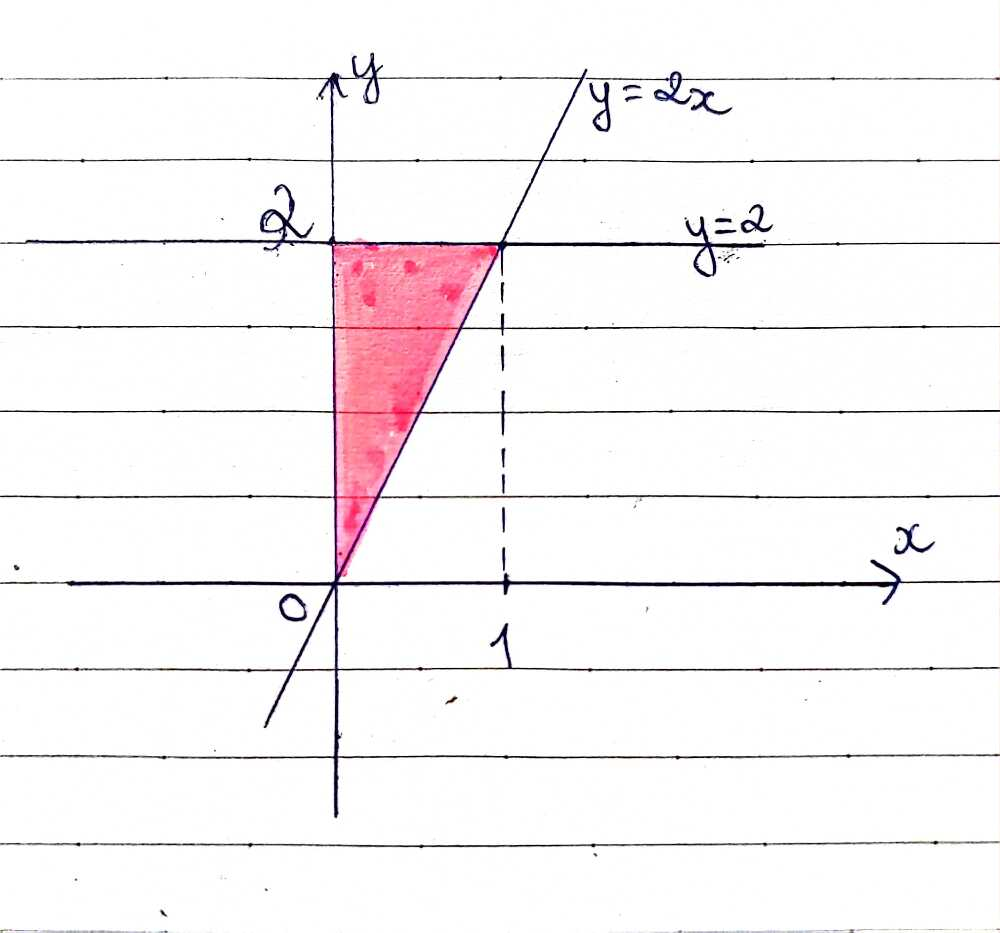
\includegraphics[width=0.5\linewidth]{ex4-1.png}
\end{center}
After sketching the domain, we will find all critical points of $f$\\
We have:\\
$f_x=4x-4\\
f_y=2y-4$\\
Consider $\left\{
\begin{array}{cr}
    f_x=0  \\
     f_y=0 
\end{array}
\right.
\iff
\left\{
\begin{array}{cr}
    4x-4=0  \\
    2y-4=0 
\end{array}
\right.
\iff
\left\{
\begin{array}{cr}
    x=1  \\
    y=2 
\end{array}
\right.\\
\Rightarrow (1,2)$ is the critical point of $f(x,y)$\\
We have: $f(1,2)=-5$\\
Then, we are going to find the boundary points of the domain where $f$ has local extreme values at these points. (Bước này tương tự như cách ta tìm Max và Min của hàm một biến)\\ In this problem, the boundaries are the lines $x=0,y=2,y=2x$.\\
+) If $x=0 \Rightarrow 0\le y \le 2$ \\(Nhìn vào domain ta vẽ, ta thấy ở trên đường $x=0$ thì y chỉ có giá trị từ 0 đến 2)\\
$\space$ $f(x,y)$ becomes $f=y^2-4y+1$\\
$\Rightarrow f'=2y-4$\\
Consider $f'=0 \iff y=2$\\
Sau đó tính $f$ tại 2 đầu mút và các critical points (điểm mà đạo hàm bằng 0 hoặc không xác định).\\
We have: (Ở đây $0\le y\le 2$ nên đầu mút là $y=0$ và $y=2$ và trùng với 1 critical point)\\
$
    f(0,0)=1\\
    f(0,2)=-3
$\\
+) If $y=2 \Rightarrow 0\le x \le 1$ (Ở trên đường $y=2$, $x$ chỉ có giá trị từ 0 đến 1)\\
$f(x,y)$ becomes $f=2x^2-4x-3$
$\Rightarrow f'=4x-4\\$
Consider $f'=0 \iff x=1$\\
We have:\\
$f(0,2)=-3\\
f(1,2)=-5$\\
+) If $y=2x \Rightarrow 0 \le x \le 1$\\
$f(x,y)$ becomes $f=6x^2-12x+1$\\
$\Rightarrow f'=12x-12$\\
Consider $f'=0 \iff x=1$\\
We have:\\
$f(1,2)=-5\\
f(0,0)=1$\\
Now, we look at all the values of $f$ we evaluated at two previous steps.\\
Finally, $f(1,2)=-5$ is the absolute minimum of $f$ and $f(0,0)=1$ is the absolute maximum of $f$.\\
\textbf{Example:} Find the absolute maximum and minimum values of $f(x,y)=48xy-32x^3-24y^2$ on the rectangle plate $0\le x\le 1$ and $0\le y\le1$.
\begin{center}
    \textbf{Solution}\\
    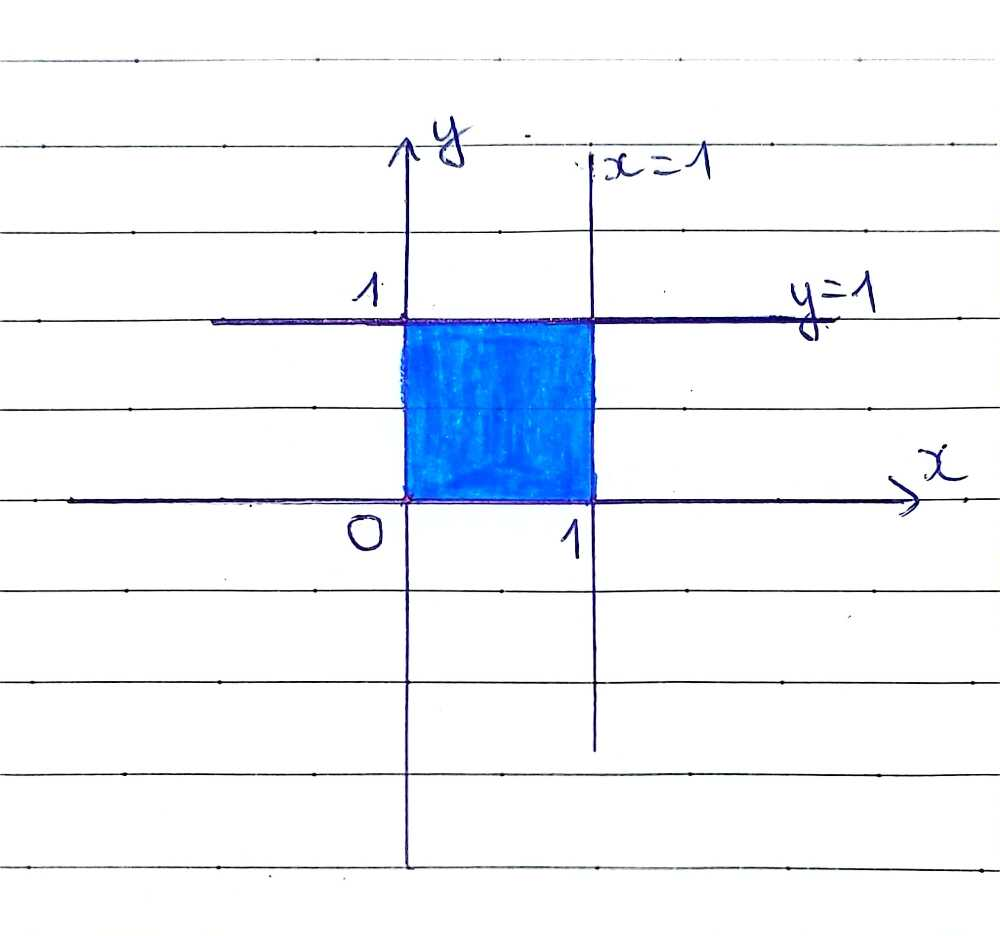
\includegraphics[width=0.45\linewidth]{4.22.png}
\end{center}
The rectangle is bounded by 4 lines: $x=0,\ x=1,\ y=0,\ y=1.$\\
We have:
\begin{center}
    $f_x=48y-96x^2$\\
$f_y=48x-48y$
\end{center}
Consider $\left\{
    \begin{array}{cr}
         f_x=0  \\
         f_y=0
    \end{array}
\right.
\iff
\left\{
    \begin{array}{cr}
         48y-96x^2=0  \\
         48x-48y=0
    \end{array}
\right.
\iff
\left\{
    \begin{array}{cc}
         -96x^2+48x&=0  \\
         x&=y
    \end{array}
\right.\\
\iff
\left\{
    \begin{array}{cr}
        \left[
         \begin{array}{cc}
              x=\displaystyle\frac{1}{2}  \\
              x=0 
         \end{array}  
         \right.\\
         x=y
    \end{array}
\right.
\iff
    \left\{\begin{array}{cr}
         x=\displaystyle\frac{1}{2}  \\
         y=\displaystyle\frac{1}{2}
    \end{array}
    \right.$ or $
    \left\{\begin{array}{cr}
         x=0  \\
         y=0
    \end{array}
    \right.\\
$
$\Rightarrow \left(\displaystyle\frac{1}{2},\frac{1}{2}\right),\ (0,0)$ are critical points of $f$.\\
We have:\\
$f\left(\displaystyle\frac{1}{2},\frac{1}{2}\right)=2\\
f(0,0)=0$\\\\
+) If $x=0 \Rightarrow 0\le y \le 1$\\
$f(x,y)$ becomes $f=-24y^2\\
\Rightarrow f'=-48y$\\
Consider $f'=0 \iff y=0$\\
We have: ($f(0,0)$ has been calculated before so we will not calculate it again)\\
$f(0,1)=-24$\\\\
+) If $x=1 \Rightarrow 0\le y\le 1$\\
$f(x,y)$ becomes $f=48y-32-24y^2\\
\Rightarrow f'= -48y+48$\\
Consider $f'=0 \iff y=1$\\
We have:\\
$f(1,0)=-32\\
f(1,1)=-8$\\\\
+) If $y=0 \Rightarrow 0\le x \le 1$\\
$f(x,y)$ becomes $f=-32x^2$\\
$\Rightarrow f'=-96x^2$\\
Consider $f'=0 \iff x=0$\\
($f(0,0)$ and $f(1,0)$ have been calculated before)\\\\
+) If $y=1 \Rightarrow 0\le x \le 1$\\
$f(x,y)$ becomes $f=48x-32x^2-24$\\
$\Rightarrow f'=-96x^2+48$\\
Consider $f'=0 \iff \left[
\begin{array}{cc}
     x=\displaystyle\frac{\sqrt{2}}{2}&  \\
      x=\displaystyle\frac{-\sqrt{2}}{2}& \text{ (not suitable)}
\end{array}
\right.$\\
We have:\\
$f\left(\displaystyle\frac{\sqrt{2}}{2},1\right)=-24+16\sqrt{2}$\\\\
Finally, $f\left(\displaystyle\frac{1}{2},\frac{1}{2}\right)=2$ is the absolute maximum of $f$ and $f(1,0)=-32$ is the absolute minimum of $f$
\newpage
\section{Double Integrals}
\subsection{Application of Calculating Volume and Area}
Consider a solid over a region R of the xy-plane.\\
Suppose $z=f(x,y)\ge 0$ is the height at each point $(x,y)\in$ R, where $f$ is a continuous function on R.\\
\textbf{- Calculating volume:}
\begin{mybox}
The \textbf{volume} of the solid above the region R and under the surface $z=f(x,y)$ is given by:
\begin{equation*}
      V=\displaystyle\iint_Rf(x,y)\ dA
\end{equation*}
\end{mybox}
\begin{center}
    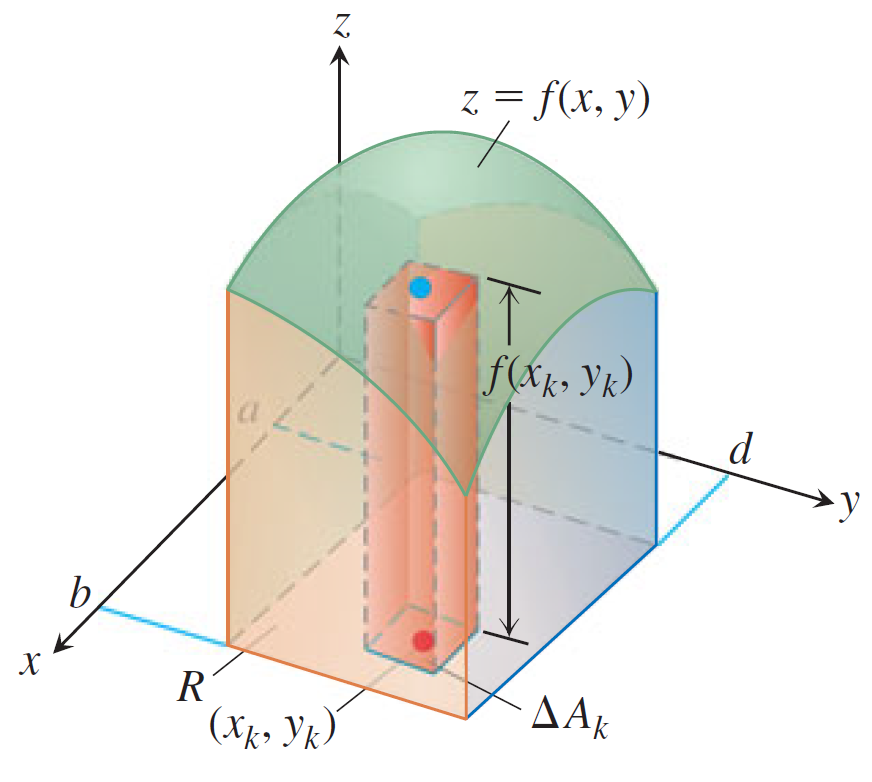
\includegraphics[width=0.45\linewidth]{vo.png}
    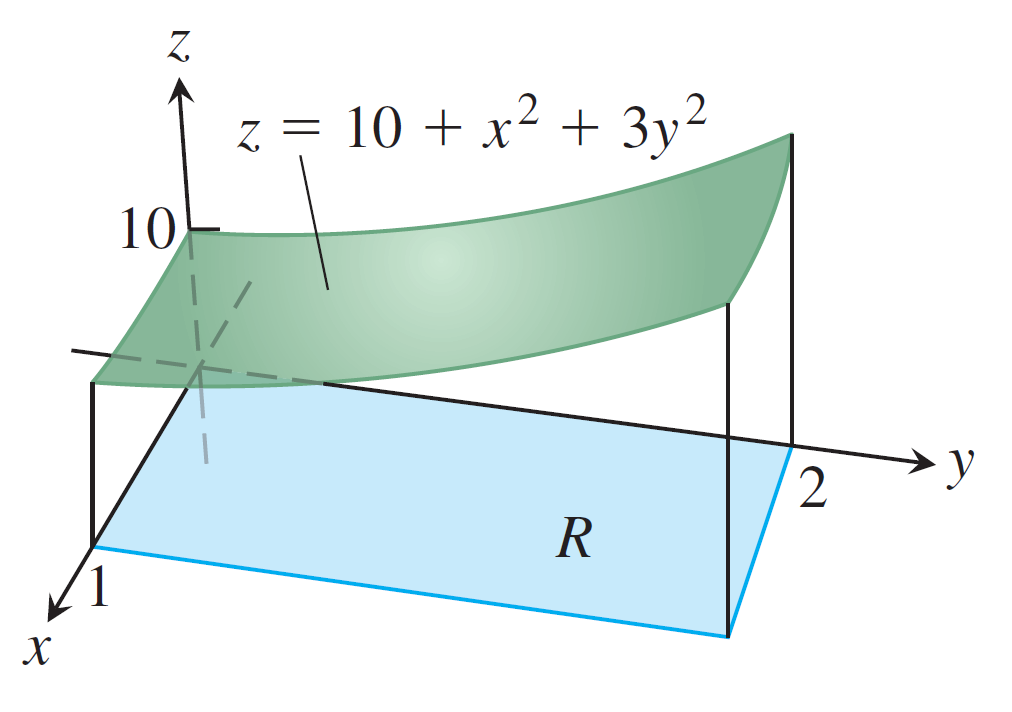
\includegraphics[width=0.45\linewidth]{volume.png}
\end{center}
\textbf{- Calculating area:}
\begin{mybox}
When $f(x,y)=1$ for all $(x,y)\in$ R, we obtain the area of R:
\begin{equation*}
      A=\displaystyle\iint_R dA
\end{equation*}
\end{mybox}
\textbf{- Average value of $z=f(x,y)$ (Average height of surface $z=f(x,y)$)  over R :}
\begin{mybox}
    \begin{center}
        \textbf{Average value} $=\displaystyle\frac{\text{volume of the solid above R and under the surface $z$}}{\text{area of R}}
        =\frac{V}{A}
        =\frac{\displaystyle\iint_R f(x,y)\ dA}{\displaystyle\iint_R dA}$
    \end{center}
\end{mybox}
\subsection{Double Integrals over Rectangles}
When the region R is a rectangle, we have this theorem:\\
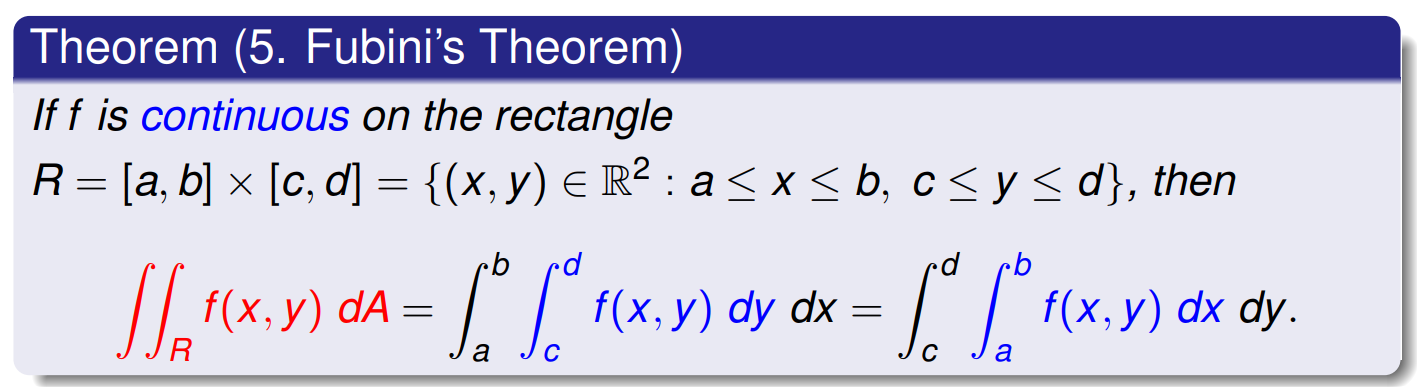
\includegraphics[width=1\linewidth]{fubini.png}\\
\textbf{Note:}\\
- Both $\displaystyle\int_a^b\int_c^df(x,y)\ dy\ dx$ and $\displaystyle\int_c^d\int_a^bf(x,y)\ dx\ dy$ are\textbf{ iterated integrals}.\\
- $\displaystyle\int_a^b\int_c^df(x,y)\ dy\ dx=\displaystyle\int_a^b\left(\int_c^df(x,y)\ dy\right)dx$ được tính bằng cách tính tích phân ở trong theo biến $y$ trước (coi $x$ là constant) sau đó tính tích phân bên ngoài theo biến $x$.\\
- $\displaystyle\int_c^d\int_a^bf(x,y)\ dx\ dy=\displaystyle\int_c^d\left(\int_a^bf(x,y)\ dx\right)dy$ được tính bằng cách tính tích phân ở trong theo biến $x$ trước (coi $y$ là constant) sau đó tính tích phân bên ngoài theo biến $y$.
\begin{center}
    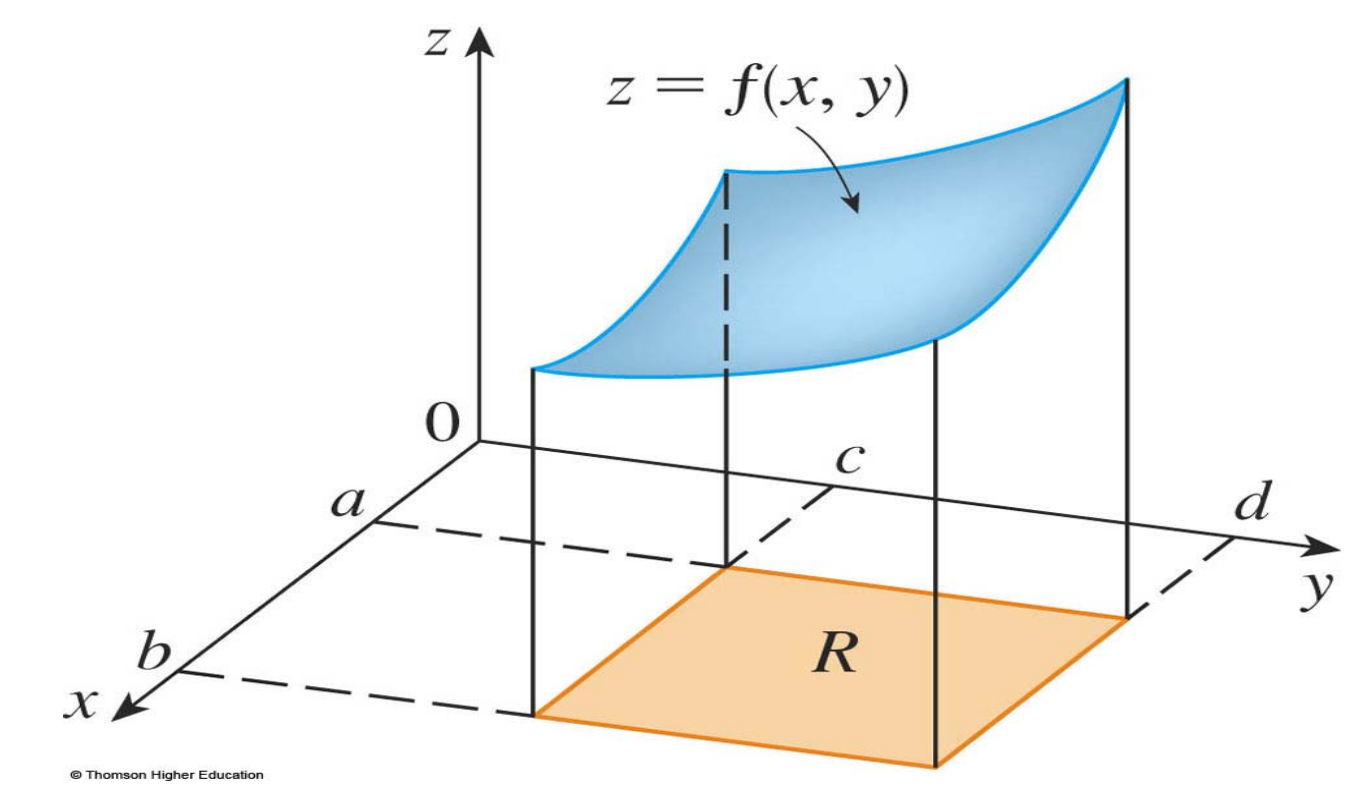
\includegraphics[width=0.5\linewidth]{rec.png}\\
    \textit{The rectangle R: $a\le x \le b$, $c\le y\le d$ (rectangular region R)}
\end{center}
\textbf{Example:} Calculate $\displaystyle\iint_Rf(x,y)\ dA$ for $f(x,y)=2xy$ and $R:\ 1\le x\le 2,\ 0\le y \le 4$
\begin{center}
    \textbf{Solution}
\end{center}
$\displaystyle\iint_Rf(x,y)\ dA=\int_1^2\int_0^42xy\ dy\ dx$\ \ \ \   or\ \ \ \ $\displaystyle\int_0^4\int_1^22xy\ dx\ dy$\\ (Cần chú ý để đúng các cận của tích phân, $dx$ đi với cận của $x$, $dy$ đi với cận của $y$)\\
I will calculate the double integral in two ways.\\
+) $\displaystyle\int_1^2\int_0^42xy\ dy\ dx
=\int_1^22x\int_0^4y\ dy\ dx$ (Vì $2x$ là const nên mình để ra ngoài)\\
$=\displaystyle\int_1^22x\left[\frac{1}{2}y^2\right]_0^4\ dx
=\int_1^2x\left[y^2\right]_0^4\ dx
=\int_1^216x\ dx
=\left[16\displaystyle\frac{x^2}{2}\right]_1^2=\left[8x^2\right]_1^2=32-8=24$\\
+) $\displaystyle\int_0^4\int_1^22xy\ dx\ dy
=\int_0^42y\int_1^2x\ dx\ dy$ (Vì $2y$ là const nên mình để ra ngoài)\\
$=\displaystyle\int_0^42y\left[\frac{1}{2}x^2\right]_1^2\ dy
=\int_0^4y\left[x^2\right]_1^2\ dy
=\int_0^43y\ dy=\left[\frac{3y^2}{2}\right]_0^4=\frac{3}{2}.16-0=24$\\
\textbf{Example:} Find the volume of the region bounded above by the surface $z=10+x^2+3y^2$ and below by the rectangle R: $0\le x \le 1,\ 0\le y\le 2$.
\begin{center}
    \textbf{Solution}
\end{center}
The volume is given by the double integral (integrate w.r.t $y$ first/tính tích phân theo biến $y$ trước):\\
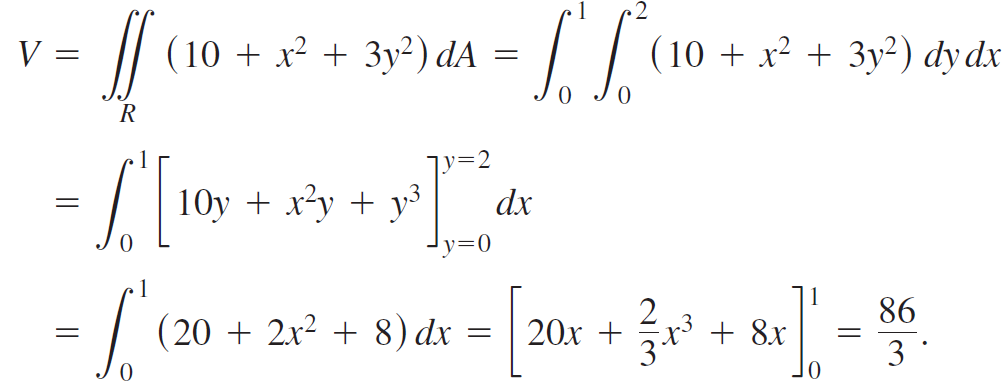
\includegraphics[width=0.6\linewidth]{sol2.png}\\
You should try integrating w.r.t $x$ first to practice.\\\\
\textbf{Example:} Calculate $\displaystyle\iint_Rf(x,y)\ dA$ which $f(x,y)=100-6x^2y$ and R: $0\le x\le 2,\ -1\le y\le 1$.
\begin{center}
    \textbf{Solution}
\end{center}
Integrate w.r.t $x$ first:\\
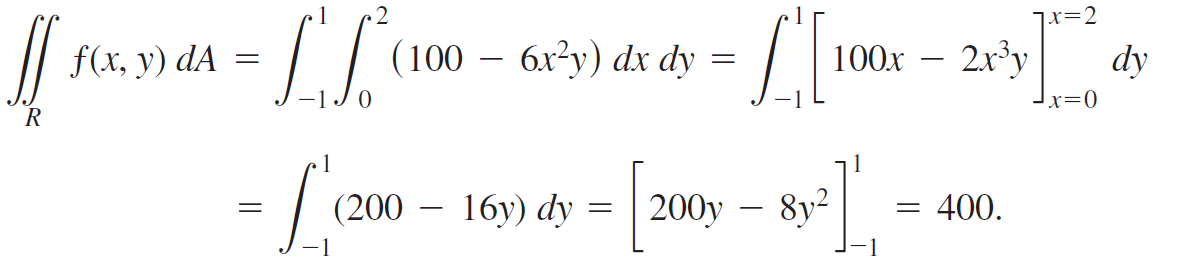
\includegraphics[width=0.65\linewidth]{sol3.png}\\
Integrate w.r.t $y$ first:\\
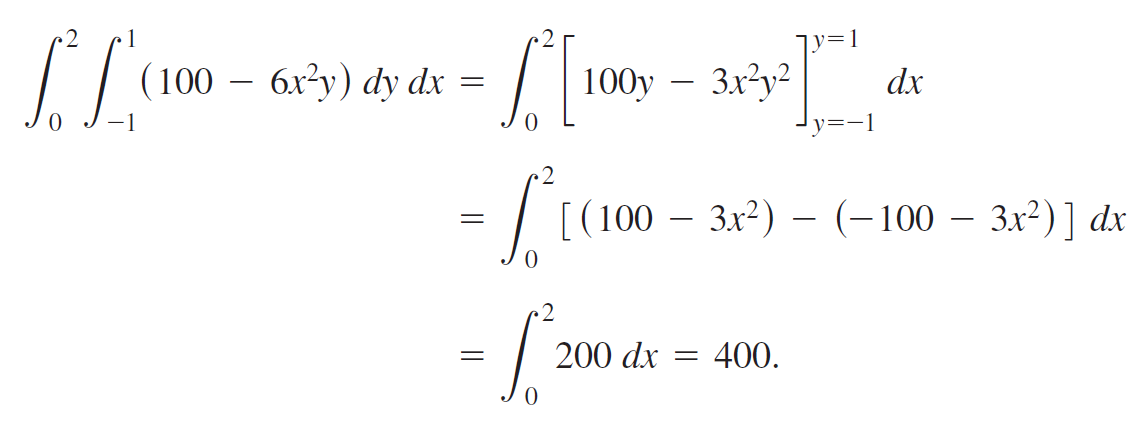
\includegraphics[width=0.65\linewidth]{sol22.png}\\
\textbf{Example:} Find the volume of the region bounded above by the surface $z =f(x,y)= 2 \sin x \cos y$ and below by the rectangle R: $0\le x\le \displaystyle\frac{\pi}{2},\ 0\le y\le\displaystyle\frac{\pi}{4}$.
\begin{center}
    \textbf{Solution}
\end{center}
The volume is obtained by the double integral:
\begin{flalign*}
    V=\displaystyle\int_0^{\pi/2}\int_0^{\pi/4}2\sin x\cos y\ dy\ dx
    =&\int_0^{\pi/2}2\sin x \left[\sin y\right]_0^{\pi/4}dx\\
    =&\int_0^{\pi/2}2.\frac{\sqrt{2}}{2}\sin x\ dx\\
    =&\int_0^{\pi/2}\sqrt{2}\sin x\ dx\\
    =&\sqrt{2}\left[-\cos x\right]_0^{\pi/2}\\
    =&\sqrt{2}
\end{flalign*}
You should try integrating w.r.t $x$ first to practice.\\
\textbf{Example: }Find the area of the rectangle R: $-1\le x\le 2,\ 0\le y\le 4$ by using double integral.
\begin{center}
    \textbf{Solution}
\end{center}
The area is obtained by this double integral:
\begin{flalign*}
     A=\displaystyle\iint_RdA
     =&\int_{-1}^2\int_0^4\ dy\ dx\\
     =&\displaystyle\int_{-1}^2\left[y\right]_0^4dx=\int_{-1}^24\ dx=[4x]_{-1}^{2}=12
\end{flalign*}
Or by this double integral:
\begin{flalign*}
    A=\displaystyle\iint_RdA
    =&\int_{0}^4\int_{-1}^2\ dx\ dy\\
    =&\int_0^4[x]_{-1}^2dy=\int_0^43\ dx=[3x]_0^4=12
\end{flalign*}
\subsection{Double Integrals over General regions}
When the region R is not a rectangle anymore, we have these theorems:
\begin{mybox}
    \textbf{[Fubini's Theorem - Stronger Form]\\Type I:} If $f(x,y)$ is continuous on a region R defined by $a\le x\le b,\ g_1(x)\le y\le g_2(x)$, with $g_1(x),\ g_2(x)$ is continuous on $\left[a,b\right]$, then
    \begin{equation*}
        \displaystyle\iint_R f(x,y)\ dA=\int_a^b\int_{g_1(x)}^{g_2(x)}f(x,y)\ dy\ dx
    \end{equation*}
\end{mybox}
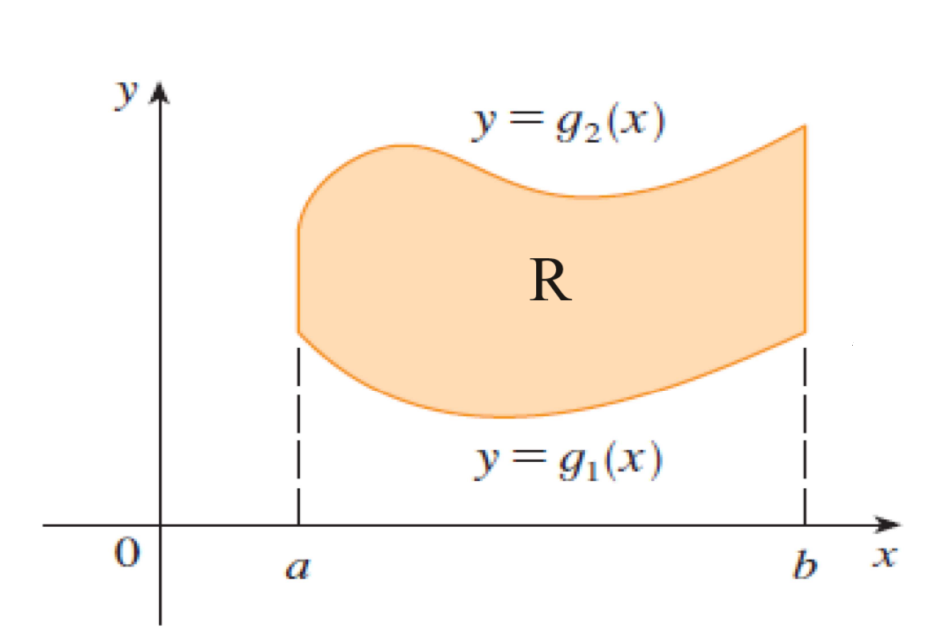
\includegraphics[width=0.35\linewidth]{genre1.png}
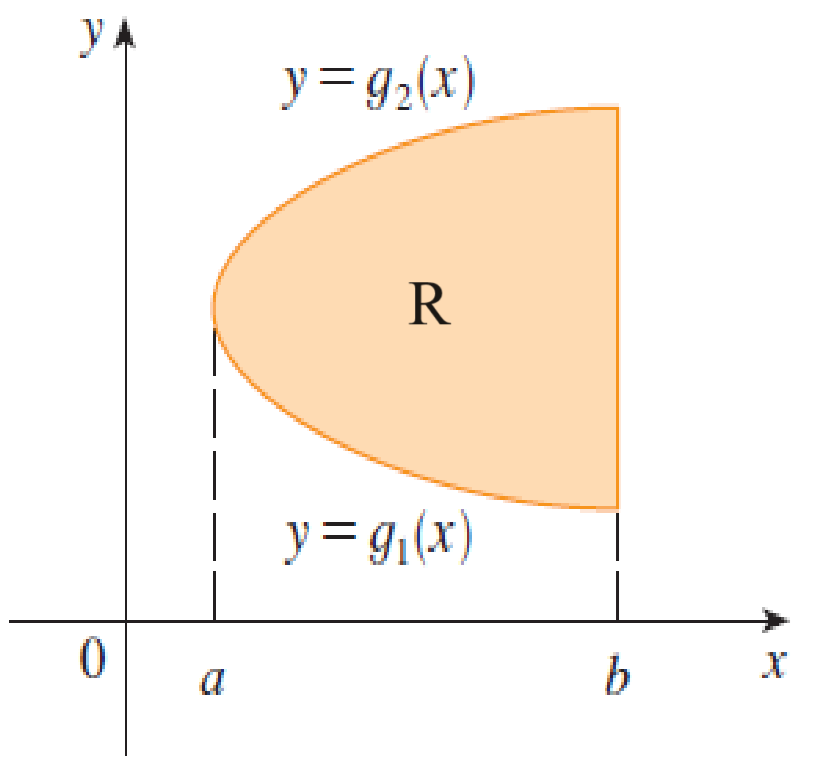
\includegraphics[width=0.25\linewidth]{genre12.png}    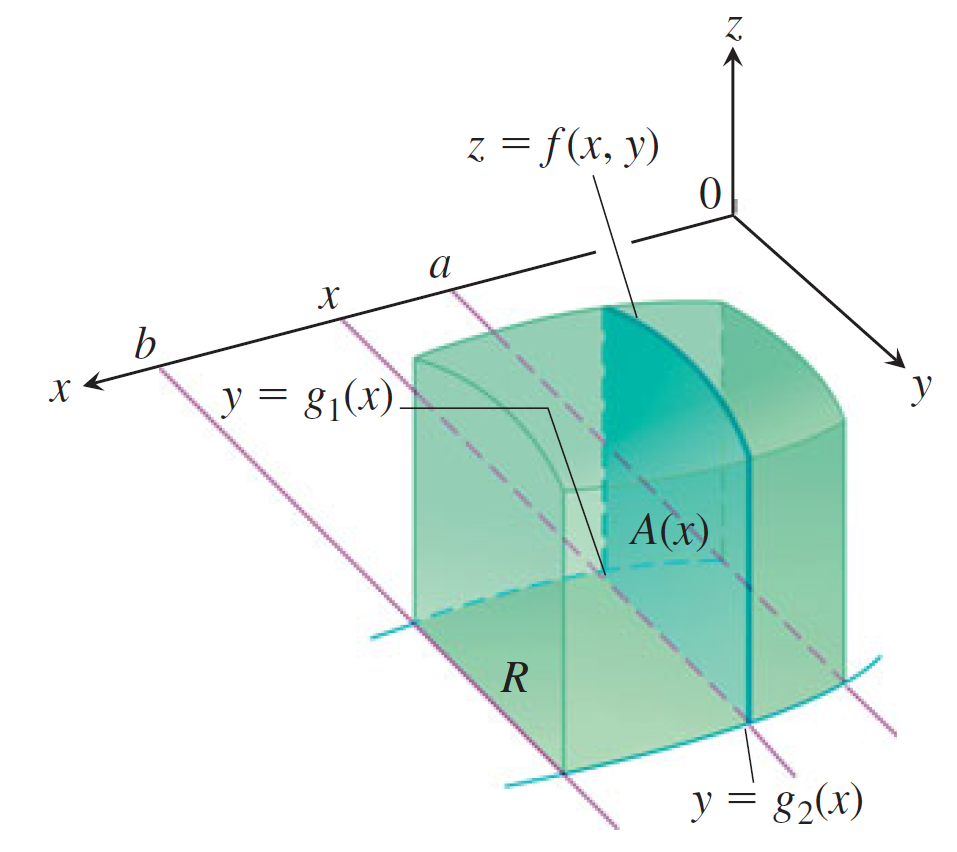
\includegraphics[width=0.35\linewidth]{type1.png}
\begin{center}
    \textit{General Region R and Diagram - Type I}
\end{center}
\begin{mybox}
    \textbf{[Fubini's Theorem - Stronger Form]\\Type II:} If $f(x,y)$ is continuous on a region R defined by $c\le y\le d,\ h_1(y)\le x\le h_2(y)$, with $h_1(y),\ h_2(y)$ is continuous on $\left[c,d\right]$, then
    \begin{equation*}
        \displaystyle\iint_R f(x,y)\ dA=\int_c^d\int_{h_1(y)}^{h_2(y)}f(x,y)\ dx\ dy
    \end{equation*}
\end{mybox}
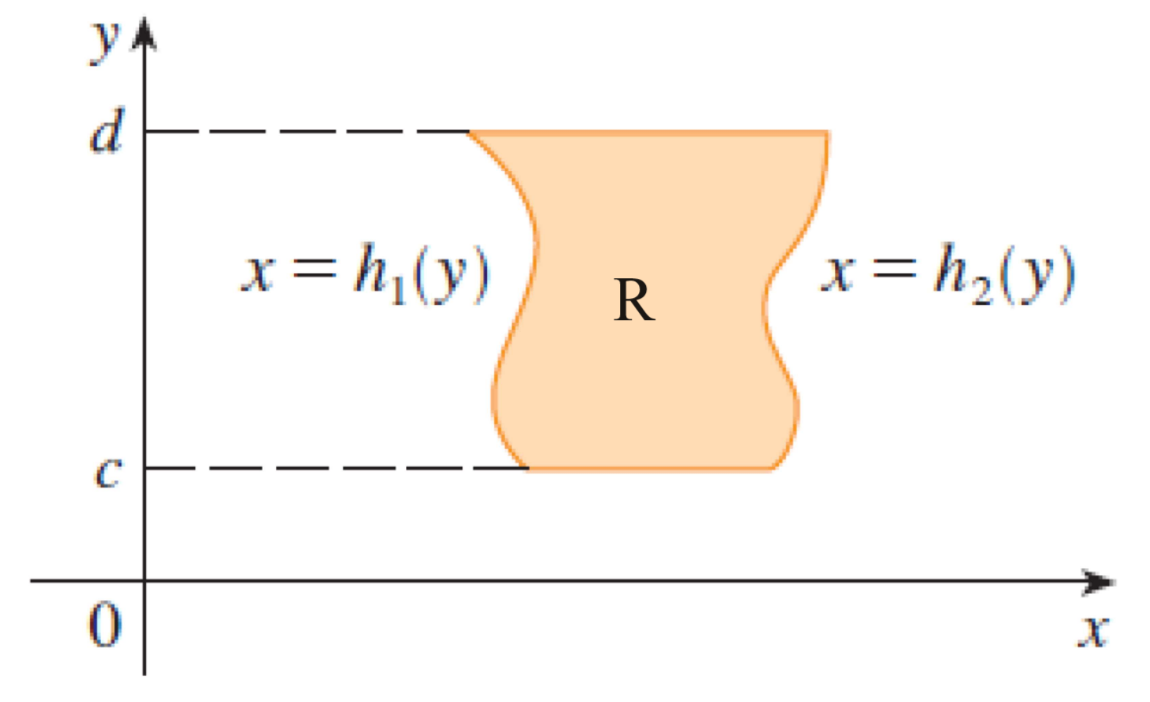
\includegraphics[width=0.35\linewidth]{genre2.png}    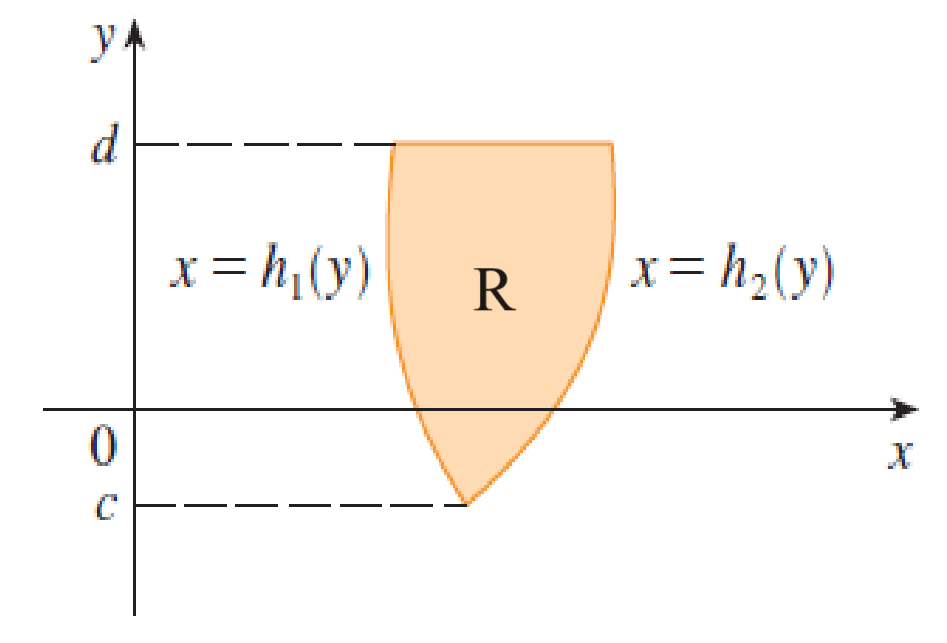
\includegraphics[width=0.35\linewidth]{genre21.png}
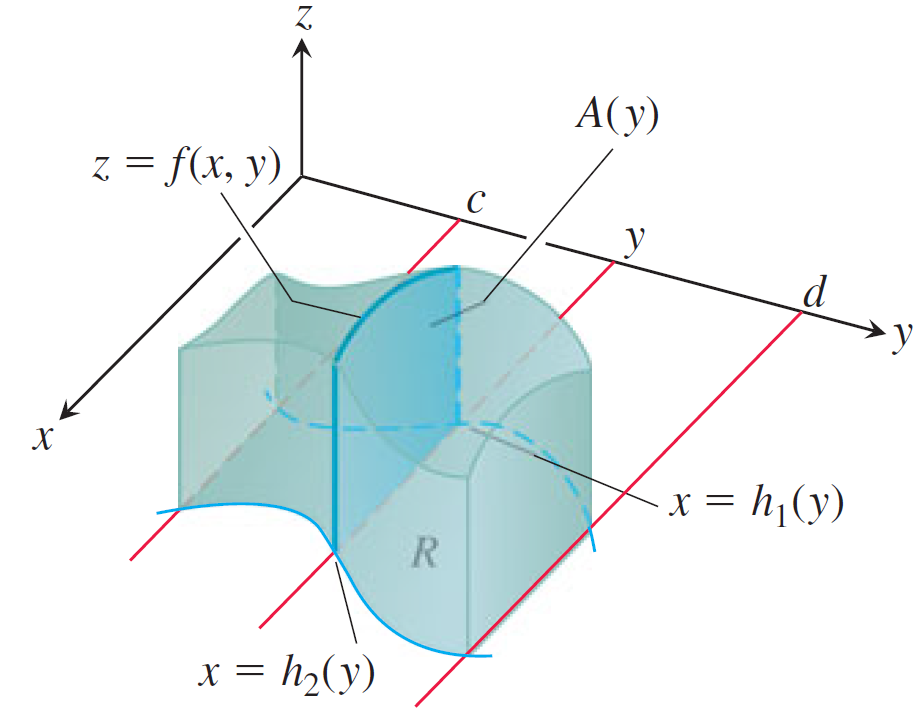
\includegraphics[width=0.35\linewidth]{type2.png}
\begin{center}
    \textit{General Region R and Diagram - Type II}
\end{center}
\textbf{Note:} To calculate these types of double integrals, you have to sketch the region R to specify the bounds $g_1(x),g_2(x),h_1(y),h_2(y)$ and find their intersections.\\
\textbf{Example:} Find the volume of the solid under the surface $z=f(x,y)=3-x-y$ and above the region R in the $xy$-plane bounded by the lines $y=0,\ y=x\text{ and }x=1$.
\begin{center}
    \textbf{Solution}
\end{center}
[Đồ thị ở trang sau...]\\
The lines $x=1$ and $y=x$ intersect each others at $(1,0)$.\\
In this problem, we can describe the region R as both type I and type II:\\
(Ta xác định hàm nào lớn hơn dựa vào chiều dương của trục $Ox$ và $Oy$)\\
- Type I: $0\le x\le 1,\ g_1(x)=0\le y\le g_2(x)=x$\\ ($g_1(x)=0\le y\le g_2(x)=x$ vì đường $y=x$ nằm phía trên đường $y=0$ (trục $Ox$))\\
- Type II: $0\le y\le 1,\ h_1(y)=y\le x\le h_2(y)=1$\\ ($h_1(y)=y\le x\le h_2(y)=1$ vì đường $x=1$ nằm bên phải đường $x=y$)\\
\begin{center}
    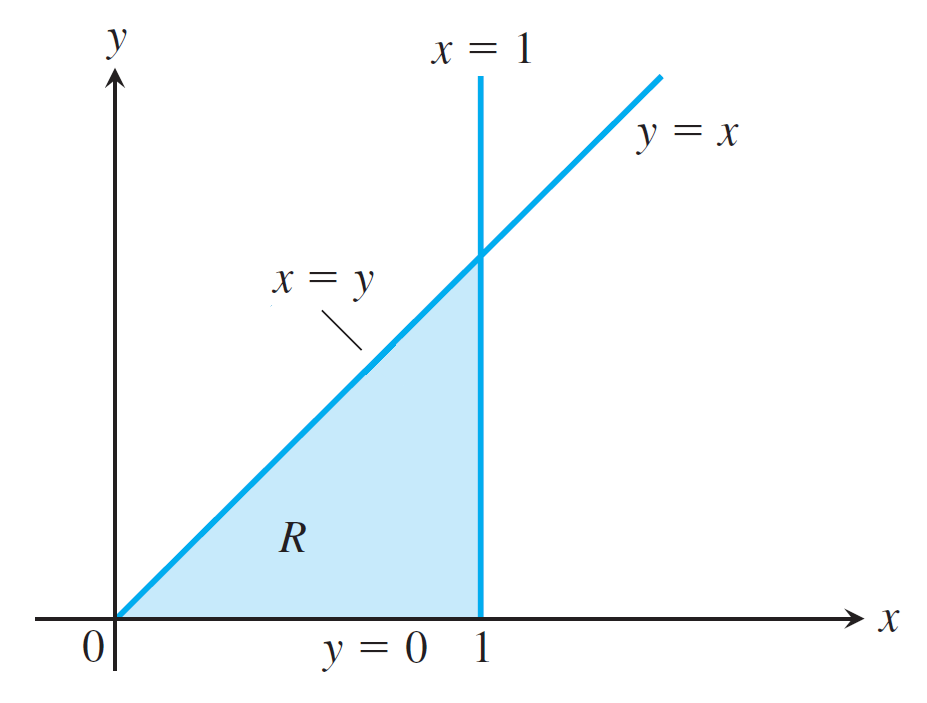
\includegraphics[width=0.4\linewidth]{so1.png}
\end{center}
The volume is obtained by the double integral (type I):
\begin{center}
    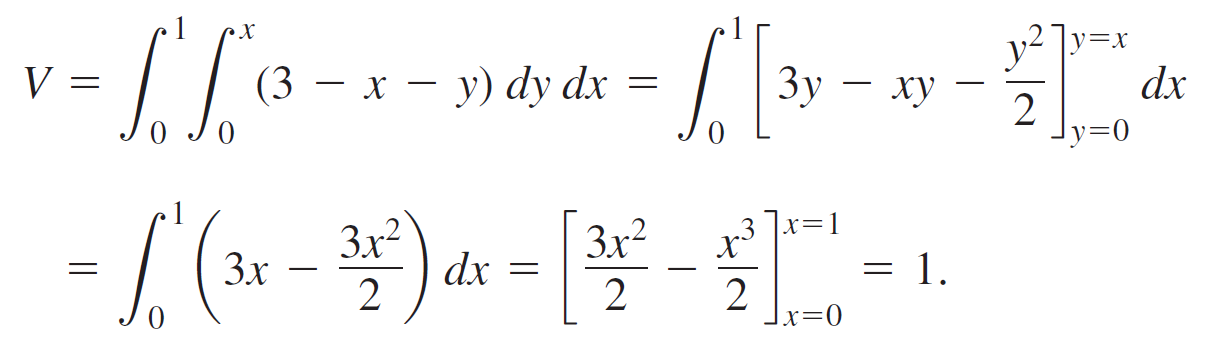
\includegraphics[width=0.6\linewidth]{sol1.png}
\end{center}
Or by the double integral (type II):
\begin{center}
    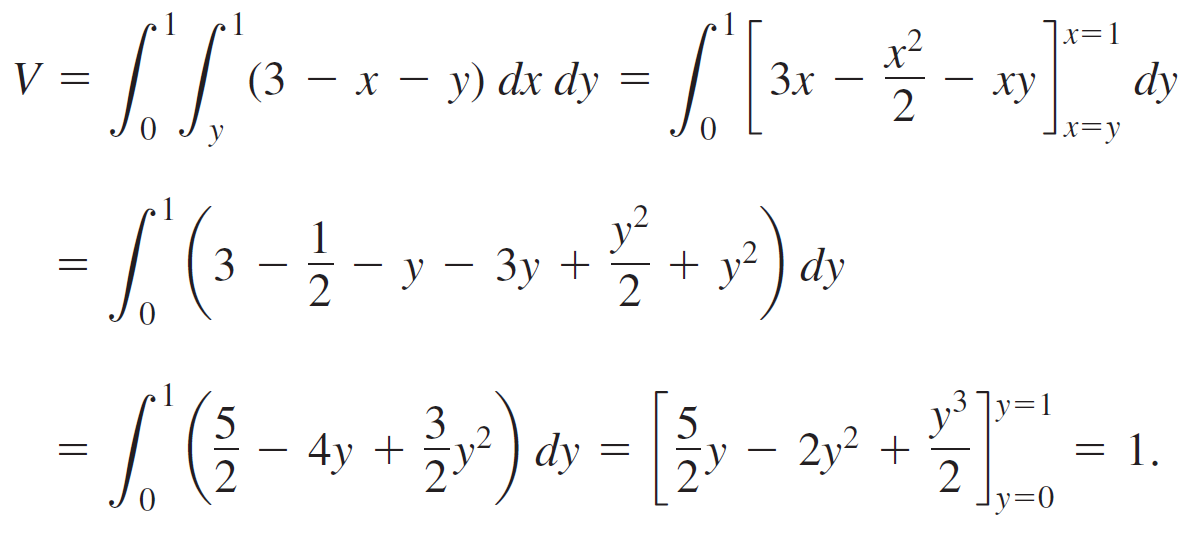
\includegraphics[width=0.6\linewidth]{sol12.png}
\end{center}
\textbf{Example: }Sketch the region and find the area of the region bounded by the parabolas $x=y^2$ and $x=2y-y^2$ using a double integral.
\begin{center}
    \textbf{Solution}
\end{center}
\begin{center}
    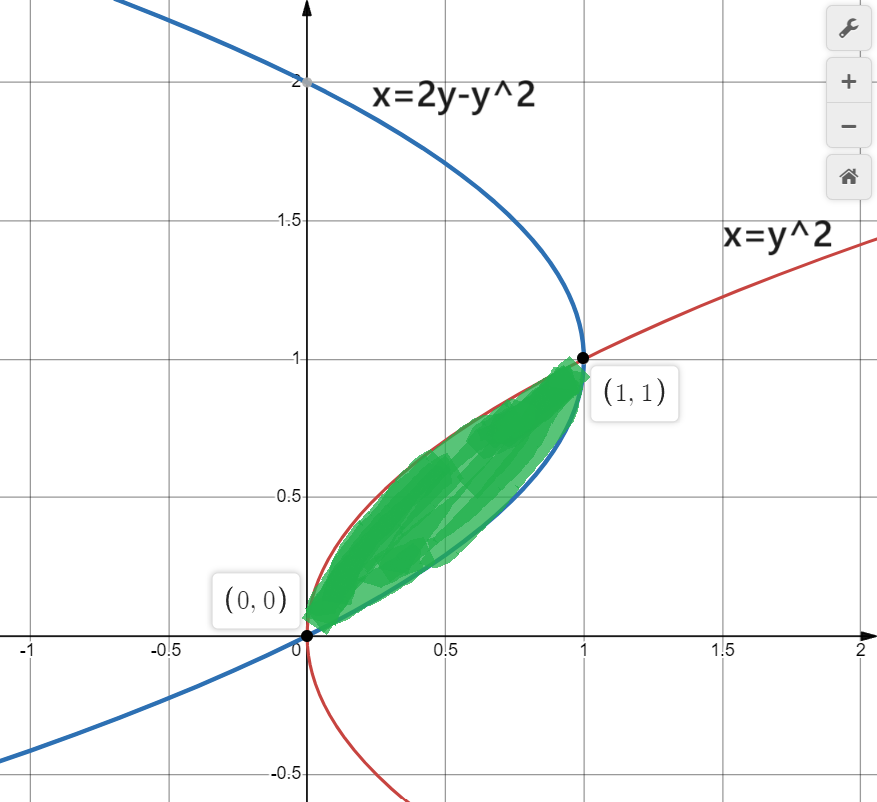
\includegraphics[width=0.45\linewidth]{R2.png}
\end{center}
The parabolas $x=y^2$ and $x=2y-y^2$ intersect each others at:\\$
\left\{
\begin{array}{cr}
     x=&y^2  \\
     x=&2y-y^2 
\end{array}
\right.
\iff
\left\{
\begin{array}{cr}
     x=&y^2  \\
     y^2=&2y-y^2 
\end{array}
\right.
\iff
\left\{
\begin{array}{cr}
     x&=y^2  \\
     2y^2-2y&=0 
\end{array}
\right.
\iff
\left\{
\begin{array}{cr}
     x=y^2  \\
     \left[
        \begin{array}{cr}
             y=0  \\
             y=1 
        \end{array}
     \right.
\end{array}
\right.
\iff
\left[
\begin{array}{cr}
     \left\{
    \begin{array}{cr}
        x=0  \\
        y=0 
    \end{array}
    \right.\\
     \left\{
    \begin{array}{cr}
        x=1  \\
        y=1 
    \end{array}
    \right.
\end{array}
\right.
$\\
$\Rightarrow$ The intersections are $(0,0),(1,1)$\\
(The region: $0\le y\le 1,\ y^2\le x\le 2y-y^2$)\\
The area is obtained by the double integral (Type II):
\begin{flalign*}
    \int_0^1\int_{y^2}^{2y-y^2}dx\ dy
    =\int_0^1[x]_{y^2}^{2y-y^2}dy
    =\int_0^1(2y-y^2-y^2)dy
    =\int_0^1(2y-2y^2)dy=\left[y^2-\displaystyle\frac{2}{3}y^3\right]_0^1=1-\frac{2}{3}=\frac{1}{3}
\end{flalign*}
(Nếu muốn tính theo type I thì ta phải biến 2 hàm số $x=y^2$ và $x=2y-y^2$ từ hàm số biến $y$ sang hàm số biến $x$ (có dạng $y=f(x)$) nên sẽ rất phức tạp.)\\
\textbf{Example: }Calculate $\displaystyle\iint_R\frac{\sin x}{x}dA$, where R is the triangle in the $xy$-plane bounded by the $x$-axis, the lines $x=y$ and $x=1$.
\begin{center}
    \textbf{Solution}
\end{center}
\begin{center}
    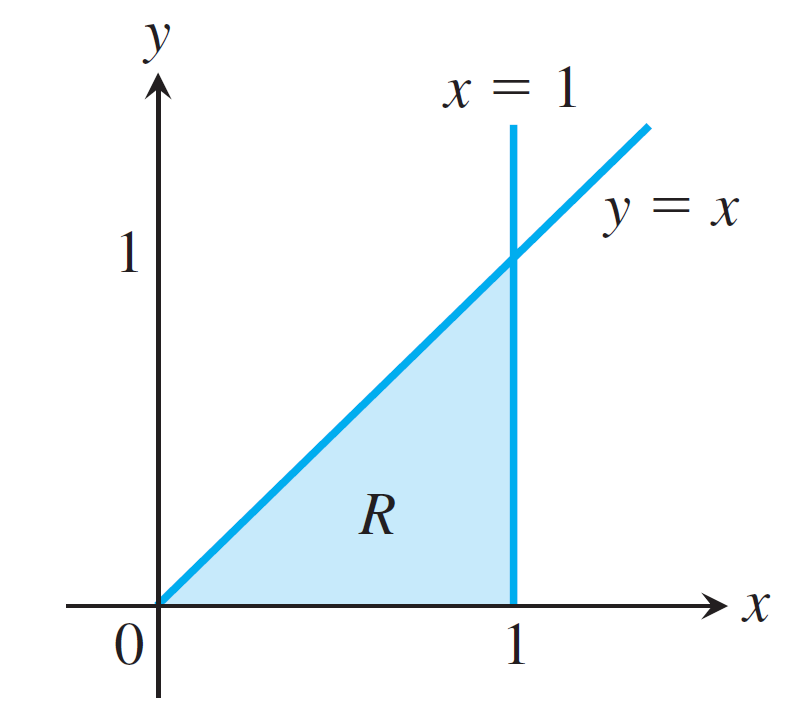
\includegraphics[width=0.4\linewidth]{so3.png}
\end{center}
The region R (Type I): $0\le x\le 1,\ 0\le y\le x$\\
The double integral becomes:
\begin{center}
        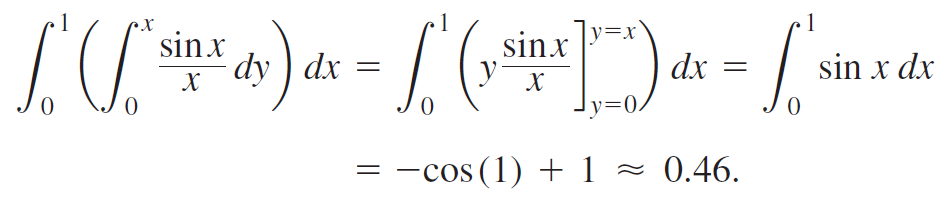
\includegraphics[width=0.6\linewidth]{so4.png}
\end{center}
The region R (Type II): $0\le y\le 1,\ y\le x\le 1$\\
The double integral becomes:
\begin{flalign*}
    \displaystyle\int_0^1\int_y^1\frac{\sin x}{x}dx\ dy
\end{flalign*}
However, $\displaystyle\int\frac{\sin x}{x}dx$ cannot be expressed in terms of elementary functions (there is no simple antiderivative).\\
There is no general rule for predicting which order of integration will be the good one in circumstances like these. If the order you first choose doesn’t work, try the other.\\\\\\\\\\
\textbf{Example:} Sketch the region of integration for the double integral
\begin{flalign*}
    V=\displaystyle\int_0^2\int_{x^2}^{2x}(4x+2)dy\ dx
\end{flalign*}
and write an equivalent integral with the order of integration reversed. Then calculate the average value of $f(x)=4x+2$.
\begin{center}
    \textbf{Solution}
\end{center}
\begin{center}
    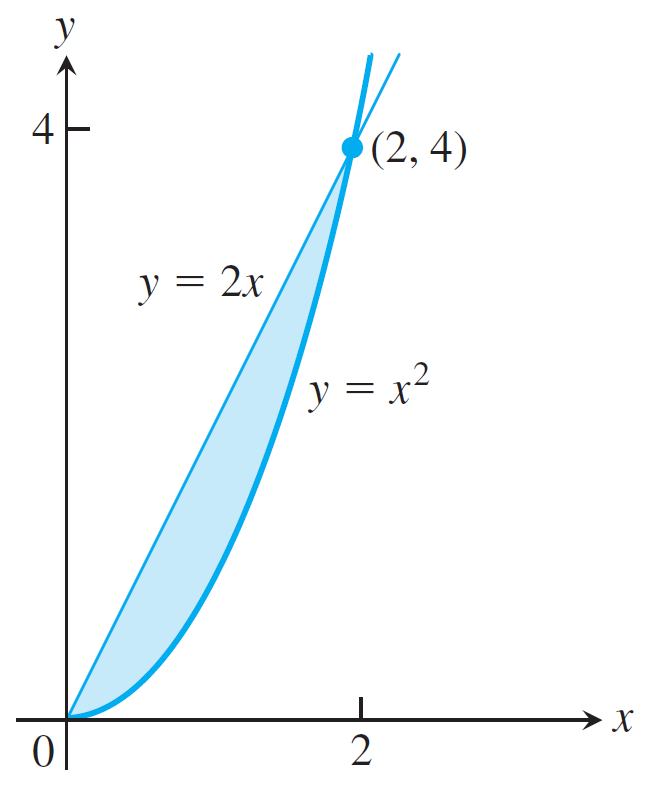
\includegraphics[width=0.3\linewidth]{so5.png}
\end{center}
The region given by the integral is: $0\le x\le 2,\ x^2\le y\le 2x$ (Type I).\\
$\Rightarrow$ The region is bounded by the line $y=2x$, the parabola $y=x^2$ and their intersections are $(0,0),(2,4)$.\\
(Để viết lại double integral này từ Type I sang Type II thì ta phải chuyển 2 hàm số $y=f(x)$ trên sang dạng hàm số $x=f(y)$).\\
For $0\le y\le 4$, we have:\\
+) $y=2x \iff x=\displaystyle\frac{y}{2}$\\
+) $y=x^2 \iff x=\sqrt{y}$\\
$\Rightarrow$ The region of type II is: $0\le y\le 4,\ \displaystyle\frac{y}{2}\le x\le \sqrt{y}$\\
$\Rightarrow V=\displaystyle\int_0^2\int_{x^2}^{2x}(4x+2)dy\ dx=\int_0^4\int_{y/2}^{\sqrt{y}}(4x+2)dx\ dy$\\
We have:
\begin{flalign*}
    V=\displaystyle\int_0^2\int_{x^2}^{2x}(4x+2)dy\ dx
    &=\int_0^2(4x+2)\left[y\right]_{x^2}^{2x}dx\\
    &=\int_0^2(4x+2)(2x-x^2)dx\\
    &=\int_0^2(-4x^3+6x^2+4x)dx\\
    &=\left[-x^4+2x^3+2x^2\right]_0^2\\
    &=8
\end{flalign*}
(You should try calculating $\displaystyle\int_0^4\int_{y/2}^{\sqrt{y}}(4x+2)dx\ dy$ to practice.)
\begin{flalign*}
    A=\displaystyle\int_0^2\int_{x^2}^{2x}dy\ dx
    =\displaystyle\int_0^2(2x-x^2)\ dx
    =\left[x^2-\frac{x^3}{3}\right]_0^2
    =\frac{4}{3}
\end{flalign*}
$\Rightarrow$ The average value of $f(x,y)=4x+2$ is $\displaystyle\frac{V}{A}=6$
\subsection{Properties of Double Integrals}
\begin{center}
    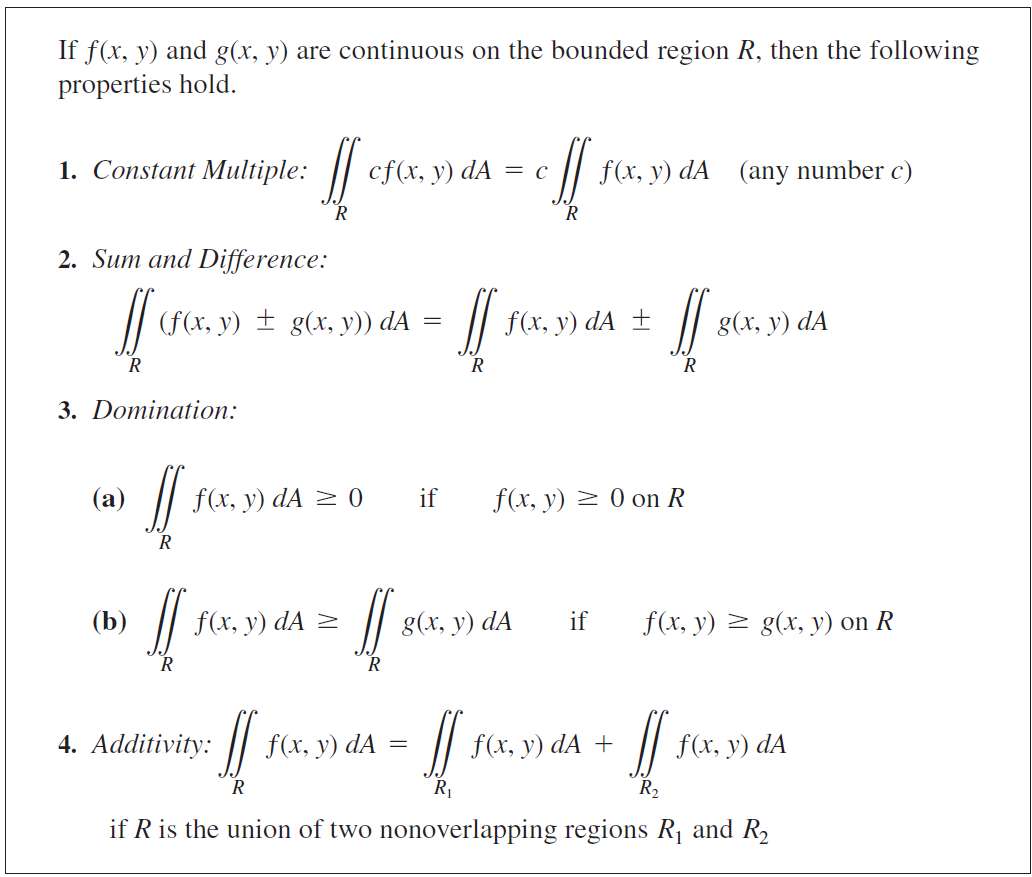
\includegraphics[width=1\linewidth]{prop.png}
\end{center}
\begin{center}
    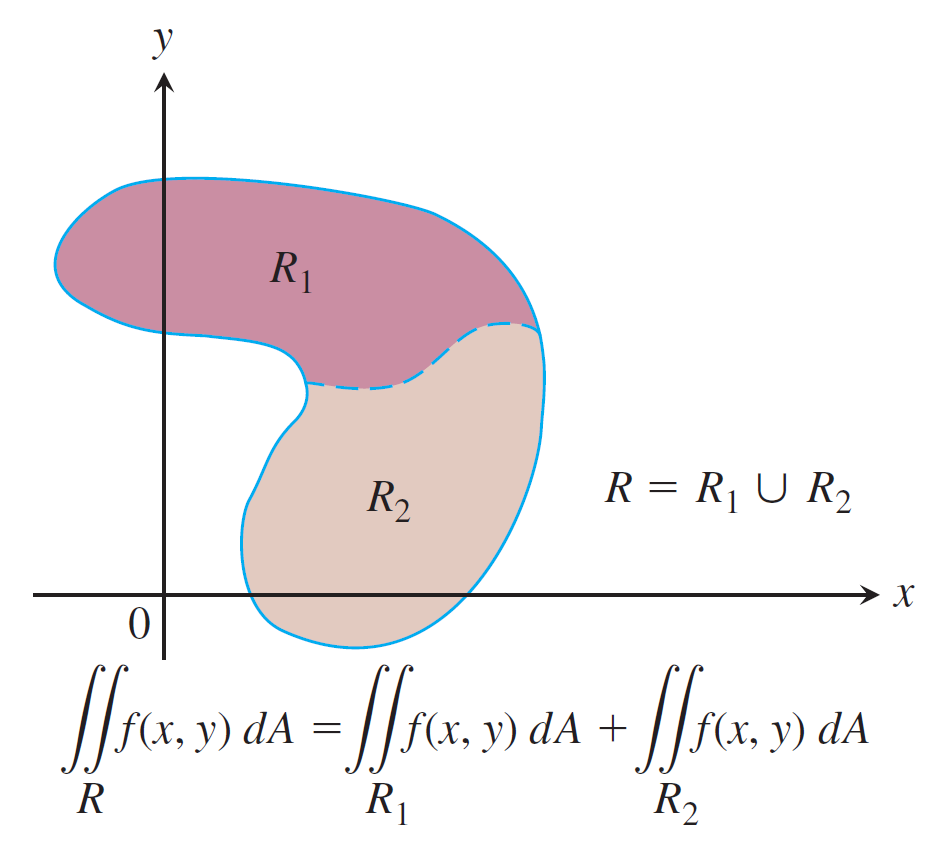
\includegraphics[width=0.5\linewidth]{propadd.png}\\
    \textit{The Additivity Property
for rectangular regions holds for regions
bounded by smooth curves}
\end{center}
\section{Optimization Problem: Lagrange Multipliers}
In optimization problems, we are looking for the largest value or the smallest value that a function can take.\\
Assume that the absolute extreme values exist, we have:\\
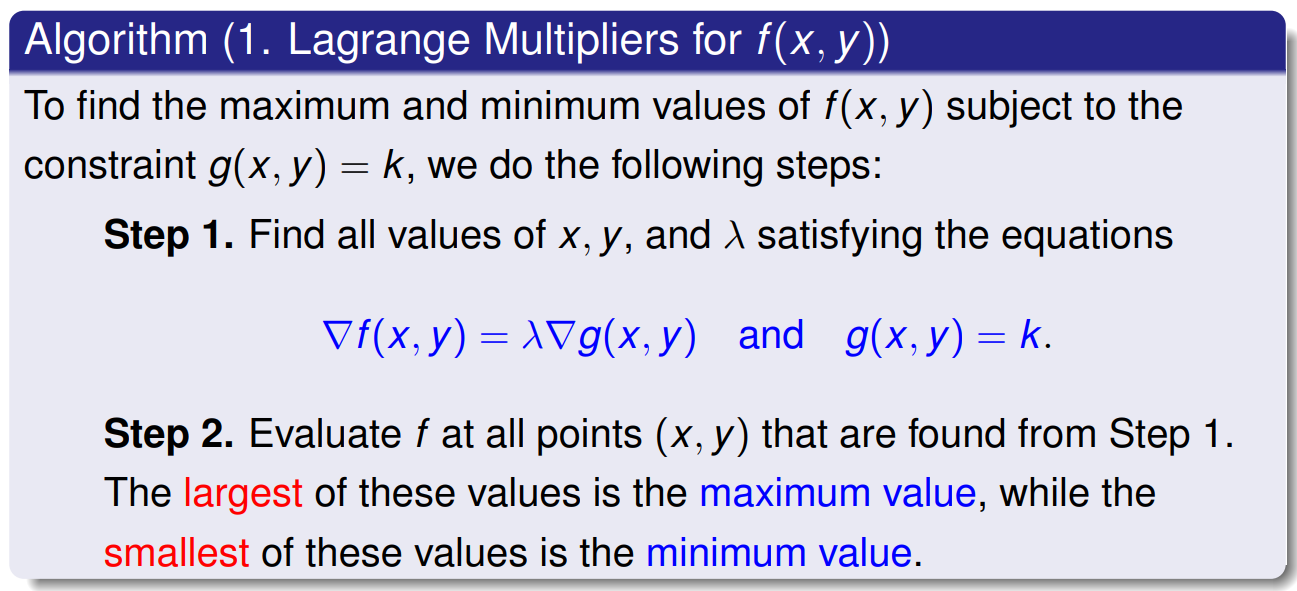
\includegraphics[width=1\linewidth]{lagrange.png}\\
\textbf{Note:} \\
- We discuss the method of Lagrange multipliers for maximizing or
minimizing a function $f(x, y)$ subject to a constraint of the form
$g(x, y) = k$. That is:
\begin{flalign*}
    \left\{
        \begin{array}{cc}
             f(x,y) \rightarrow \text{max/min}  \\
             g(x,y) =k 
        \end{array}
    \right.
\end{flalign*}
- If $\lambda =0$, then $\nabla f(x,y)$ gives stationary points of $f$.\\
- If $\lambda \ne 0$, then both vectors $\nabla f(x,y)$ and $g(x,y)$ are parallel or opposite each to other.\\
- The Algorithm for functions of three variables is the same as for functions of two variables, adding the third variable $z$.\\\\
\textbf{Example: }Find the local extreme values of $f(x,y)=x^2y$ on the line $x+y=3$.
\begin{center}
    \textbf{Solution}
\end{center}
We have:\\
$f_x=2xy\\
f_y=x^2\\
\Rightarrow \nabla f=(2xy,x^2)$\\
We have:\\
$g(x,y)=x+y\\
g_x=1\\
g_y=1\\
\Rightarrow \nabla g=(1,1)$\\
Consider: 
$\left\{
\begin{array}{cr}
     \nabla f=\lambda \nabla g\\
     g(x,y)=3 
\end{array}
\right.
\iff 
\left\{
\begin{array}{cr}
     (2xy,x^2)=\lambda (1,1)\\
     x+y=3 
\end{array}
\right.
\iff 
\left\{
\begin{array}{cr}
     2xy=\lambda  \\
     x^2=\lambda\\
     y=3-x
\end{array}
\right.
\iff 
\left\{
\begin{array}{cr}
     2x(3-x)=x^2  \\
     x^2=\lambda\\
     y=3-x
\end{array}
\right.\\
\iff 
\left\{
\begin{array}{cr}
     3x^2-6x=0  \\
     x^2=\lambda\\
     y=3-x
\end{array}
\right.
\iff 
\left\{
\begin{array}{cr}
     \left[
     \begin{array}{cc}
          x=2\\
          x=0
     \end{array}
     \right.  \\
     x^2=\lambda\\
     y=3-x
\end{array}
\right.
\iff
\left[
\begin{array}{cc}
     \left\{
        \begin{array}{cc}
             x=0\\
              y=3\\
              \lambda=0
        \end{array}
     \right.\\
      \left\{
        \begin{array}{cc}
             x=2\\
              y=1\\
              \lambda=4
        \end{array}
     \right.
\end{array}
\right.\\
\Rightarrow f(0,3)=0$ and $f(2,1)=4$ are local extreme values of $f=x^2y$ on the line $x+y=3$\\\\\\
\textbf{Example: }Find the maximum and minimum values of the function $f(x,y) =3x + 4y$ on the circle $x^2 + y^2 = 1$.
\begin{center}
    \textbf{Solution}
\end{center}
We have:\\
$f_x=3\\
f_y=4\\
\Rightarrow \nabla f=(3,4)$\\
We have:\\
$g(x,y)=x^2+y^2\\
g_x=2x\\
g_y=2y\\
\Rightarrow \nabla g=(2x,2y)$\\
Consider: 
$\left\{
\begin{array}{cr}
     \nabla f=\lambda \nabla g\\
     g(x,y)=1 
\end{array}
\right.
\iff
\left\{
\begin{array}{cr}
     (3,4)=\lambda (2x,2y)\\
     x^2+y^2=1 
\end{array}
\right.
\iff
\left\{
\begin{array}{cr}
     3=2\lambda x&\\
     4=2\lambda y&\text{ ($\lambda$ always $\ne 0$)}\\
     x^2+y^2=1& 
\end{array}
\right.\\
\iff
\left\{
\begin{array}{cr}
     x=\displaystyle\frac{3}{2\lambda x}\\\\
     y=\displaystyle\frac{2}{\lambda}\\\\
     x^2+y^2=1 
\end{array}
\right.
\iff
\left\{
\begin{array}{cr}
     x=\displaystyle\frac{3}{2\lambda x}\\\\
     y=\displaystyle\frac{2}{\lambda}\\\\
     \displaystyle\frac{9}{4\lambda^2}+\displaystyle\frac{4}{\lambda^2}=1 
\end{array}
\right.
\iff
\left\{
\begin{array}{cr}
     x=\displaystyle\frac{3}{2\lambda x}\\\\
     y=\displaystyle\frac{2}{\lambda}\\\\
     \lambda=\displaystyle\frac{5}{2} \text{ or } \lambda=\displaystyle\frac{-5}{2}
\end{array}
\right.\\
$
+) $\lambda=\displaystyle\frac{5}{2} \Rightarrow (x,y)=\left(\displaystyle\frac{3}{5},\frac{4}{5}\right)
\Rightarrow f\left(\displaystyle\frac{3}{5},\frac{4}{5}\right)=5$\\
+) $\lambda=\displaystyle\frac{-5}{2} \Rightarrow (x,y)=\left(\displaystyle\frac{-3}{5},\frac{-4}{5}\right)
\Rightarrow f\left(\displaystyle\frac{-3}{5},\frac{-4}{5}\right)=-5$\\
$\Rightarrow\ f\left(\displaystyle\frac{3}{5},\frac{4}{5}\right)=5$ is the absolute maximum value of $f$ and $f\left(\displaystyle\frac{-3}{5},\frac{-4}{5}\right)=-5$ is the absolute minimum value of $f$ on the the circle $x^2+y^2=1$.
\newpage
\begin{center}
    \textbf{FEEDBACK FOR THIS DOCUMENT}\\
    
\includegraphics[width=0.5\linewidth]{qr.png}\\
    \textbf{Please scan this QR code...}\\
    \textbf{Or click this link:} \url{https://forms.gle/qmMhmKmVWHVKNAaG6} \\
    to give us feedback on this document!!!
\end{center}
Please spend a little time to send your feedback. Although it is just a simple work, it has great significance to us. Your feedback can help us improve our future documents and it let us know whether you understand what we have written in this document. Thank you so much for using our documents!\\
\begin{center}
    Good luck with your exam!
\end{center}
\end{document}